%%%%%%%%%%%%%%%%%%%%%%%%%%%%%%%%%%%%%%%%%%%%%%%%%%%%%%%%%%%%%%%%%%%%%%%%%%%%%%%%
%% Nature Communications manuscript: generative wall turbulence
%% Main text is split by journal section to keep figure/prose consistency
%% reviewable. The active evidence set contains eight main figures, two tables and
%% one algorithmic display.
%%%%%%%%%%%%%%%%%%%%%%%%%%%%%%%%%%%%%%%%%%%%%%%%%%%%%%%%%%%%%%%%%%%%%%%%%%%%%%%%
\documentclass[pdflatex,sn-nature]{sn-jnl}

\usepackage{graphicx}
\usepackage{multirow}
\usepackage{amsmath,amssymb,amsfonts}
\usepackage{amsthm}
\usepackage{mathrsfs}
\usepackage[title]{appendix}
\usepackage{xcolor}
\usepackage{textcomp}
\usepackage{manyfoot}
\usepackage{booktabs}
\usepackage{array}
\usepackage{algorithm}
\usepackage{algpseudocode}
\usepackage{placeins}
\usepackage{url}
\hypersetup{
  hypertexnames=false,
  bookmarksdepth=2,
  pdftitle={An interface framework and adequacy standard when generative turbulence models hit the wall},
  pdfauthor={Jianou Jiang, Haolang Zhu, Sungjong Joo, Peidong Huang, and Budimir Rosic},
  pdfkeywords={turbulence; near-wall modelling; generative modelling; flow separation}
}

\newcommand{\Rsep}{R^2_{\mathrm{sep}}}
\newcommand{\yB}{y_{\mathcal B}}
\newcommand{\Rfluct}{R^2_{\mathrm{fluct}}}
\newcommand{\ES}{\mathrm{ES}}
\newcolumntype{P}[1]{>{\raggedright\arraybackslash}p{#1}}

\raggedbottom
\renewcommand{\topfraction}{0.92}
\renewcommand{\bottomfraction}{0.90}
\renewcommand{\textfraction}{0.06}
\renewcommand{\floatpagefraction}{0.75}
\setcounter{topnumber}{2}
\setcounter{totalnumber}{3}

\begin{document}

% TITLE: 13 words. The 7 August supervisor revision adds the recurring-wall
% framing; the 10 August meeting locked "interface framework" so the first
% offered item carries its own noun and cannot be read as "interface standard".
\title[Generative turbulence models at the wall]{An interface framework and adequacy standard when generative turbulence models hit the wall}

% CORRESPONDING AUTHOR: moved to J.J. on the supervisor's instruction, 5 Aug 2026;
% address confirmed by the author 5 Aug 2026.
\author*[1]{\fnm{Jianou} \sur{Jiang}}\email{jianou.jiang@eng.ox.ac.uk}
\author[1]{\fnm{Haolang} \sur{Zhu}}
\equalcont{These authors contributed equally and share second authorship.}
\author[1]{\fnm{Sungjong} \sur{Joo}}
\equalcont{These authors contributed equally and share second authorship.}
\author[1]{\fnm{Peidong} \sur{Huang}}
\equalcont{These authors contributed equally and share second authorship.}
\author[1]{\fnm{Budimir} \sur{Rosic}}
\equalcont{These authors contributed equally and share second authorship.}

\affil*[1]{\orgdiv{Department of Engineering Science}, \orgname{University of Oxford},
\orgaddress{\street{Parks Road}, \city{Oxford}, \postcode{OX1 3PJ},
\country{United Kingdom}}}

\abstract{Generative models are gaining attention in fluid mechanics amid hopes of a step
change in turbulence modelling from whole-field reconstruction. Yet they inherit the
century-old difficulty of computational fluid dynamics: representing the near-wall region.
It occupies little volume yet sets drag, separation, wall-generated vorticity and
loads. Volume-averaged training and validation objectives weight its cells by count, not dynamical leverage. We identify why the commonly used wall-closure
interface fails and build one that works. Expanding predicted wall stress into an
equilibrium-law velocity band destroys the information; through a conditioning slot
the generator was trained to read, the stress propagates. Across a bluff-body cube array,
attached channel and separating periodic hill---the cube and hill deliberately difficult
engineering flows---cube viscous wall-force error falls by
two-fifths, the channel recovers
three-quarters of the exact-traction benefit, and the hill transmits in one of two generative
families. The result is an interface framework and adequacy standard: an equal-footing slot that delivers any wall model's stress to the generator undistorted, and an oracle control certifying whether a generative family detects wall information, offered to refocus generative turbulence modelling on the wall. Evaluations are offline
and a priori. Code and controls are available at
\url{https://github.com/JianouJiang/generative-wall-turbulence}.}

\maketitle

\section{Introduction}\label{sec:intro}

Modern turbulence modelling has changed its mathematics---from Prandtl's boundary-layer
construction, through Reynolds-averaged and large-eddy simulation, to learned generative
fields---but it keeps reaching the same physical obstacle: the wall
\cite{prandtl1904,pope2000,piomelli2002wall,bose2018wmles}. A geometrically thin near-wall layer
sets skin friction; reversal of wall shear
accompanies separation; and the resulting vorticity, shear layers and wakes organise flow well
beyond it \cite{schlichting2017boundary,pope2000}. Coherent near-wall motions sustain turbulence,
while outer scales partly predict them at high Reynolds number
\cite{robinson1991coherent,jimenez1999autonomous,mathis2009amplitude,marusic2010predictive,smits2011highre,lee2015direct}. Resolving this
small region dominates simulation cost at engineering Reynolds numbers
\cite{chapman1979computational,choi2012grid}; conventional simulation has therefore spent
decades coupling unresolved wall physics to a resolved outer flow
\cite{schumann1975subgrid,cabot2000approximate,larsson2016wmles}. Generative models do not escape
that physics simply by learning the field.

Machine learning now supplies data-driven closures, solver acceleration and learned operators
\cite{ling2016reynolds,duraisamy2019turbulence,kochkov2021machine,brunton2020machine,vinuesa2022enhancing,li2021fno,lu2021deeponet}.
Generative families represent whole-field distributions for inflow, wakes, reconstruction,
super-resolution and subfilter closure
\cite{goodfellow2014gan,ho2020ddpm,song2021sde,karras2022edm,lipman2023flow,
kim2020deep,drygala2022generative,lienen2024zero,buzzicotti2021reconstruction,stengel2020adversarial,bode2021piesrgan,kohl2024benchmarking,dong2025stochclosure},
with conditional variants reconstructing fields from partial observations
\cite{chung2023dps,song2023pigdm,wang2023ddnm,shu2023pidiffusion,rybchuk2023}. Yet two properties
create a wall-specific failure mode: neural networks preferentially fit low-frequency,
large-scale content \cite{rahaman2019spectral,oommen2026learning}, and a volume-averaged loss
weights a thin wall band by cell count rather than by dynamical leverage. A boundary-localised
error can therefore contribute little to a global objective while materially changing drag or
separation (Supplementary Table~13). Validation inherits the same weighting: a volume-averaged
score can certify a reconstruction whose implied wall stress is wrong. Wall treatment is not a
niche refinement of a whole-field
model; it limits what that model can establish wherever surface forces matter.

Representative whole-field formulations are not universally wall-blind: Gao \emph{et al.}
generate wall-bounded fields
\cite{gao2023bayesian}; CoNFiLD includes periodic-hill, rough-wall and channel cases and
documents larger discrepancies near the wall \cite{du2024confild}; Oommen \emph{et al.} address
super-resolution, forecasting and sparse reconstruction
\cite{fukami2019jfm,fukami2021nmi,kim2021unsupervised,oommen2026learning}. Our concern
is not that wall-bounded examples are absent, and we are not claiming that machine learning
universally ignores walls. Yet whole-field objectives do not by
themselves give a thin wall region its engineering weight, and none has an explicit
wall-closure-to-generator interface.

Wall-focused work provides important counterexamples: early neural models of near-wall
turbulence \cite{milano2002neural}, turbulent fields estimated from wall shear and pressure
\cite{guastoni2021convolutional,guemes2021coarse,cuellar2024three}, low-order wall-bounded
surrogates \cite{srinivasan2019predictions,nakamura2021convolutional}, learned synthetic inflow
\cite{wu2017inflow,fukami2019synthetic,kim2020deep}, conditional flow matching from wall
observations \cite{parikh2026conditional} and latent-diffusion wall-pressure reconstruction
\cite{fan2025wallpressure}. In parallel, wall models represent the unresolved near-wall layer for
large-eddy simulation \cite{kawai2012wall,yang2015integral,park2014improved,yang2017llm,bae2019dynamic},
including machine-learning wall models \cite{yang2019predictive,bae2022scientific} extended to
pressure-gradient and separated regimes \cite{lozanoduran2023building,dupuy2023wallmodel}. The
strands answer different questions---which field is compatible with supplied wall data, versus
which unresolved surface quantity can be supplied to a resolved computation---and neither role
substitutes for the other in a coupled simulation.

Two things are missing between them. There is no tested \emph{interface}: no whole-field generative
formulation takes its wall boundary from a closure---generative models have
produced closure terms \cite{dong2025stochclosure}, not consumed a wall model's output---and
no wall closure has been judged by what a generator can propagate from it. And there is no \emph{standard} for testing one---no agreed way
to show that a record can detect wall information at all before it is used to argue that wall
information does or does not matter. Without that, a generative model responding to nothing and a
wall channel carrying nothing produce the same measurement.

\begin{figure}[t]
\centering
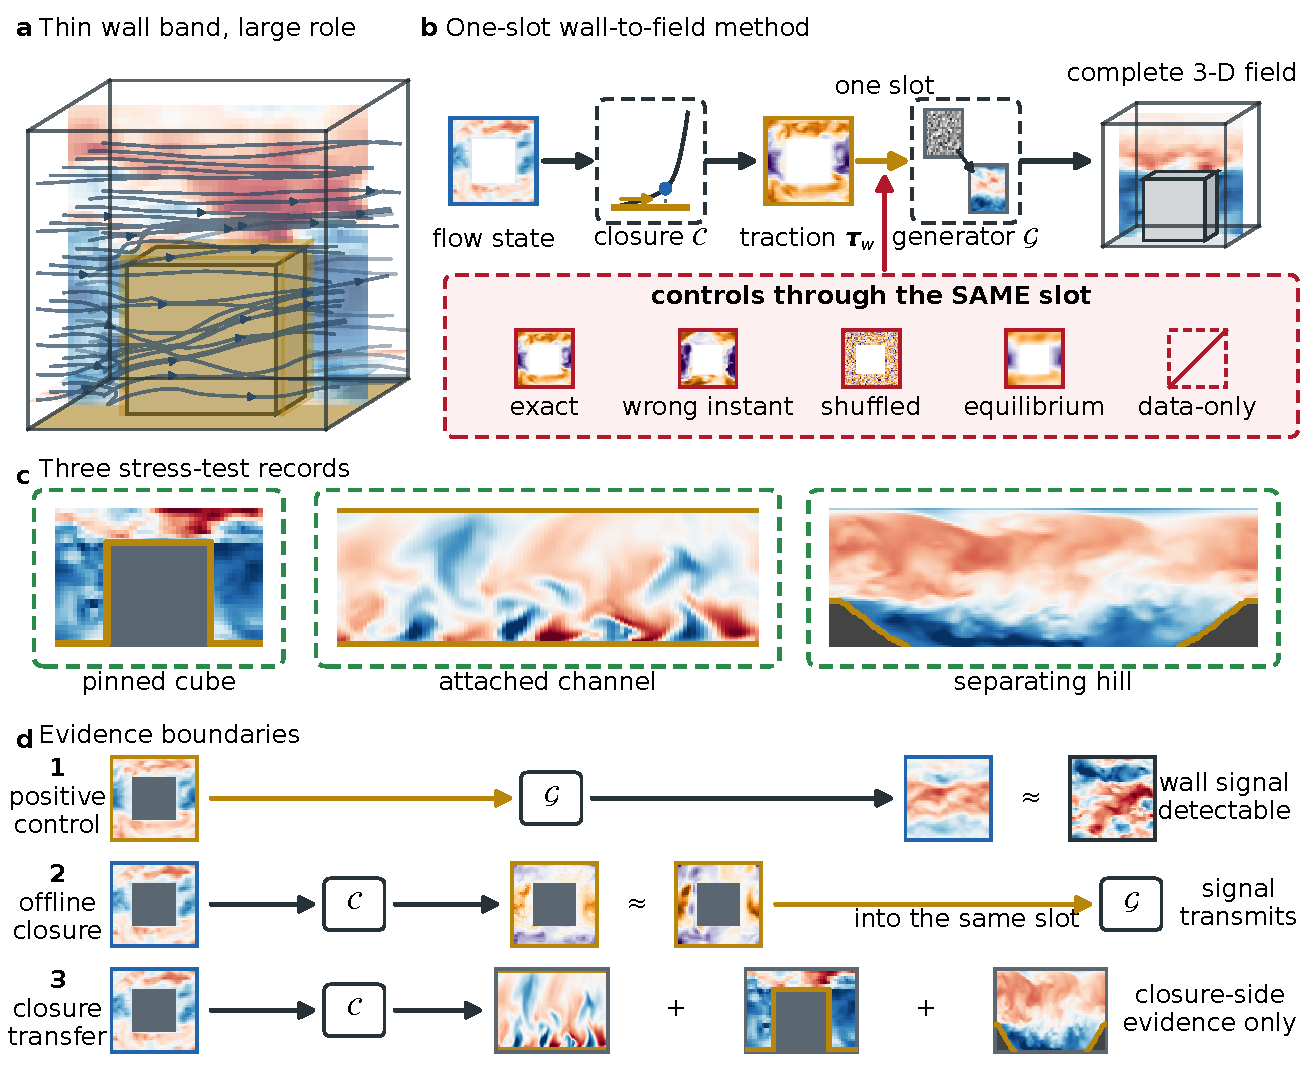
\includegraphics[width=\linewidth]{figures/fig1_architecture.pdf}
\caption{\textbf{Why generative turbulence models need an explicit wall interface.}\enspace
\textbf{a}, The thin supplied near-wall band (gold) wraps the floor and cube while its influence
is assessed through the surrounding three-dimensional field.
\textbf{b}, The one-slot method: matching-height flow state enters closure $\mathcal C$, whose
signed traction $\boldsymbol{\tau}_w$ conditions generator $\mathcal G$; every wall model and
control enters through this same slot. \textbf{c}, Three deliberately distinct stress tests and
their qualitative outcomes: the pinned cube shows field and wall-load response, the attached
channel reaches positive absolute skill, and the separating hill transmits only in diffusion and
remains indicative. \textbf{d}, Evidence boundaries: the oracle band is the
positive control, the fitted closure tests offline composition
(Figs~\ref{fig:generation}--\ref{fig:slot}), and separate frozen models provide closure-side
transfer only. No row represents solver-coupled deployment.}\label{fig:arch}
\end{figure}
\FloatBarrier

This paper supplies both through three linked tests of one integrated
closure-to-generative-field system: diagnose failure of an equilibrium-band adapter, repair the
interface by conditioning directly on signed surface traction, and
standardise the positive control needed to establish that a record and generator can detect wall
information. Every wall model enters one conditioning slot without generator-side exposure, so
models are scored on equal footing. We also measure the fidelity needed for reconstruction benefit
and provide a leakage-free public-corpus protocol. Figure~\ref{fig:arch} contrasts thin support
with field influence (\textbf{a}), shows the one-slot method (\textbf{b}), identifies the stress
tests and outcomes (\textbf{c}), and separates oracle detectability, offline composition and
closure-only transfer (\textbf{d}). All evaluations are offline and a priori: no momentum equation
is advanced, and oracle observations, closure outputs and solver deployment are distinct evidence.

The records are deliberately distinct: a geometrically pinned aligned-cube array, an attached
channel and pressure-gradient-induced separation over a periodic hill. The cube and hill are
difficult engineering regimes, not flattering selections. Expanding predicted stress into an
equilibrium-law velocity band destroys the signal, whereas direct signed traction transmits
$0.63$ of a matched oracle ceiling. Closure-predicted traction then improves the source-excluded
cube field by $+0.061\,[0.057,0.064]$ and cuts inferred viscous
wall-force error by two-fifths. The
channel reaches positive absolute skill through the equal-footing slot (Fig.~\ref{fig:slot}). On
the hill, diffusion gains $+0.062\,[+0.017,+0.106]$ but carries roughly three effective samples;
the preregistered flow-matching arm fails its positive control. Complete-volume cube skill remains
negative.

Records enter the claim set only after source validation: one public record whose offline
composition initially appeared favourable is excluded because its primary source identifies it as
a two-dimensional irregular pipe with stochastic forcing \cite{du2024confild}, contradicting the
wall geometry assumed (Supplementary Note~8). Companion results evaluate the closure alone and are
preserved byte-for-byte without revalidation.

\section{Results}\label{sec:results}

\subsection{An oracle near-wall band changes the field outside it}\label{sec:cube}\label{sec:first}

The foreground flow is an aligned-cube large-eddy simulation (LES) \cite{coceal2006aligned,coceal2007cubes,xie2006les} with
plan solidity $\lambda_p=0.25$ and $Re_h=5000$---exposed floor, ceiling and cube surfaces rather
than a stack of homogeneous planes (native first-cell $y^+\leq1.92$; Methods). Of 1,101
post-spin-up fields, 660 train, 98 are excluded, and 160 temporally correlated, thinned fields are
evaluated from the chronologically separated remainder. ``LES reference'' denotes this numerical record,
not ground truth: the case has no experimental benchmark or grid/filter study.

The supplied band contains 14,008 of 207,360 fluid cells ($6.8\%$; $4.5\%$ excluding two
computational-lid strips), so the complete endpoint scores 93.24\% of the fluid domain; near and
farther endpoints split the unsupplied cells at $d/h=0.5$, a geometric label, not an
equilibrium-layer claim. The intervention is rich---a dense oracle velocity band, not wall
pressure, shear or a closure output---and tests whether a conditional generator changes outside
the supplied support given time-aligned wall information. The far-time control shifts that
band by $\approx1.40$ integral times at unchanged support and density.

The chronological allocation was recorded before any wall-arm output existed (Supplementary
Note~1). Three sequential configurations of the \emph{same} three-dimensional U-Net were run, called M0, M1 and M2. They differ only in size and budget: M0 width 24 and 30,000
updates; M1 width 48, 90,000 updates and a longer sampler; M2 differs from M1 only in using
circular padding in the two periodic directions. What separates them evidentially matters more:
M0 provided the only pre-output contact with the evaluation interval, so it is the first-contact
comparison, while M1 and M2 reused that interval and are development sensitivities, not
independent confirmations.

On the complete support-excluded volume M0 gives aligned-band $\Rfluct=0.103$, against
$-0.072$ for the absent-band branch of the same network and $-0.204$ for a far-time band:
paired gains of $+0.175$ and $+0.307$, larger near the wall, with farther-from-wall absolute
skill negative (Supplementary Table~2). M1 and M2 preserve the ordering (complete gains
$0.174$, $0.197$), but the farther-from-wall paired interval crosses zero for M1, so no
model-independent outer effect is established.

\begin{table}[t]
\caption{\textbf{Valid retained controls that delimit attribution.} All values are fluctuation
$R^2$ in the complete/near/farther-from-wall regions. These later controls use the same chronological
allocation but different estimators or training protocols from M0; they are scope tests, not a
clean numerical leaderboard.}\label{tab:controls}
\centering
\small
\begin{tabular*}{\linewidth}{@{\extracolsep{\fill}}P{6.6cm}rrr@{}}
\toprule
Estimator and information & Complete & Near & Farther \\
\midrule
Linear/Wiener, no band & $-0.00008$ & $-0.00001$ & $-0.00018$ \\
Linear/Wiener, near-wall band & $-0.05068$ & $+0.02997$ & $-0.13327$ \\
Deterministic direct band, seed 2234 & $+0.05523$ & $+0.15647$ & $-0.04842$ \\
Deterministic direct band, seed 3234 & $+0.05803$ & $+0.16121$ & $-0.04762$ \\
Nearest training band, associated field & $-0.80255$ & $-0.73251$ & $-0.87430$ \\
M0 learned absent-band arm & $-0.07240$ & $-0.07669$ & $-0.06804$ \\
\bottomrule
\end{tabular*}
\end{table}
\FloatBarrier

Table~\ref{tab:controls} delimits attribution: no estimator matched to M0's architecture, budget
and selection protocol was run, so generator superiority is not established; a frozen-record
retrieval diagnostic is strongly negative in every region, rejecting literal retrieval though not
more flexible memorisation; and a support-contaminated interior comparison is quarantined
(Supplementary Note~1). The selected M2
endpoint is not an untouched held-out test.

Figure~\ref{fig:generation} makes the intervention spatially concrete. Panel \textbf{a} fixes the
first evaluated M2 target before output inspection and pairs its contemporaneous band with an
equal-support donor 172 stored fields later. Panels \textbf{b},\textbf{c} compare the LES section,
three eight-sample arm means and their absolute errors on common scales. The aligned arm reduces
error most visibly beside the floor and cube. The mean profiles remain similar (\textbf{d}), but
the wall-normal profile resolves the local difference (\textbf{e}): aligned has the lowest
near-wall error and complete-volume RMSE, $0.112$ against $0.128$ absent and $0.136$ far-time.
This is a reconstruction benefit rather than merely a shifted mean profile. Because it shows one
target from development-contacted M2, the display illustrates rather than independently tests the
aggregate result.

Figure~\ref{fig:point} separates mechanism from evidential claim. Panels \textbf{a},\textbf{b}
map where correct-time information reduces squared error: improvement clusters around the floor
and cube but is not uniform in the outer flow. Panel \textbf{c} holds the M2 U-Net and eight noise
seeds fixed while only wall information changes; panel \textbf{d} removes supplied support before
defining complete, near and farther scores, and distinguishes absolute fluctuation $R^2$ from
paired $\Delta R^2$. Panels \textbf{e},\textbf{f} then return to first-contact M0: aligned skill is
$0.103$ complete, $0.243$ near and $-0.040$ farther, while gains over absent/far-time are
$0.175/0.307$, $0.320/0.564$ and $0.028/0.044$, respectively. Thus the wall signal is strongest
near its support; the small positive farther contrasts do not produce positive outer absolute
skill. Only terminal M0 aggregates survive, so points are shown without unreplayable intervals.

\begin{figure}[t]
\centering
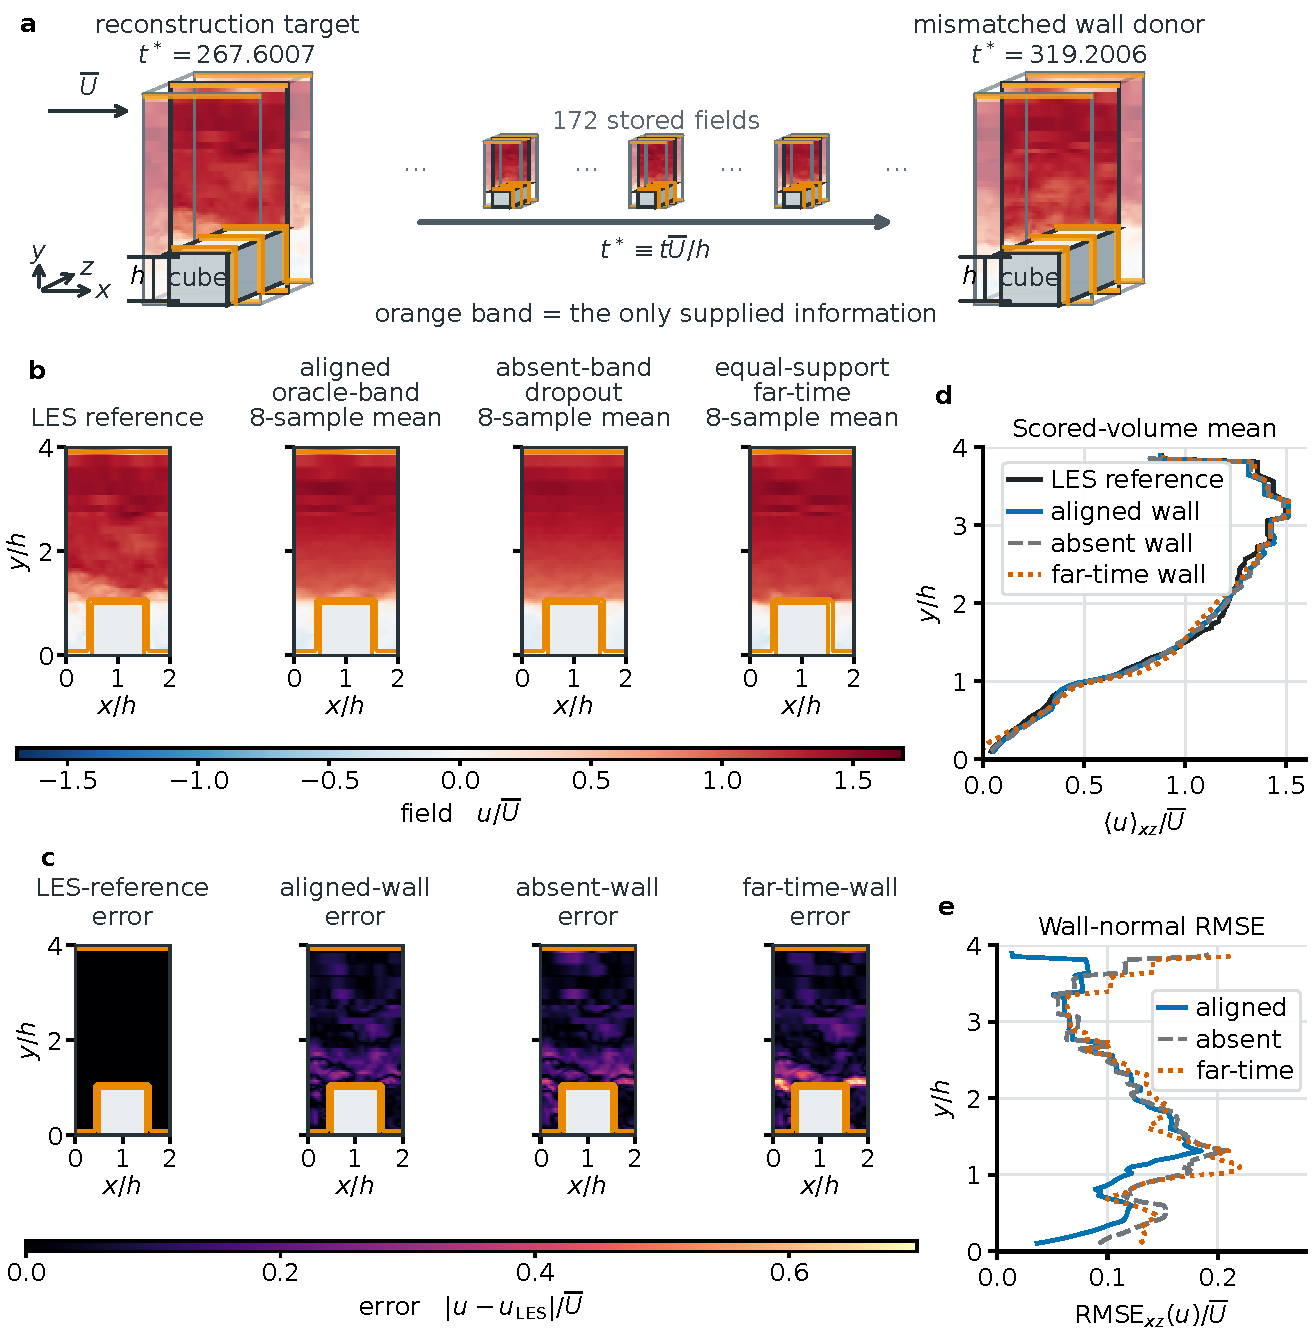
\includegraphics[width=\linewidth]{figures/fig2_generation.pdf}
\caption{\textbf{Representative aligned-cube reconstruction.}
\textbf{a}, First evaluated M2 LES target (record 758, $t\overline U/h=267.6$), fixed in
advance by the protocol rather than chosen visually, with three retained intermediate fields and
far-time wall donor (record 930); ellipses denote omitted fields. Each cutaway shows three
$x$--$y$ sections (dark: mid-span); orange marks the supplied near-wall band.
\textbf{b}, Mid-span LES reference and aligned-band, absent-band and far-time eight-sample means.
\textbf{c}, Absolute errors. \textbf{d}, Scored-volume mean profile. \textbf{e}, Wall-normal
root-mean-square error (RMSE) profile; complete-volume RMSE $0.112$ (aligned), $0.128$
(absent), $0.136$ (far-time).
One target is shown; aggregate results use 160 temporally correlated three-component fields.}
\label{fig:generation}
\end{figure}
\FloatBarrier

\begin{figure}[t]
\centering
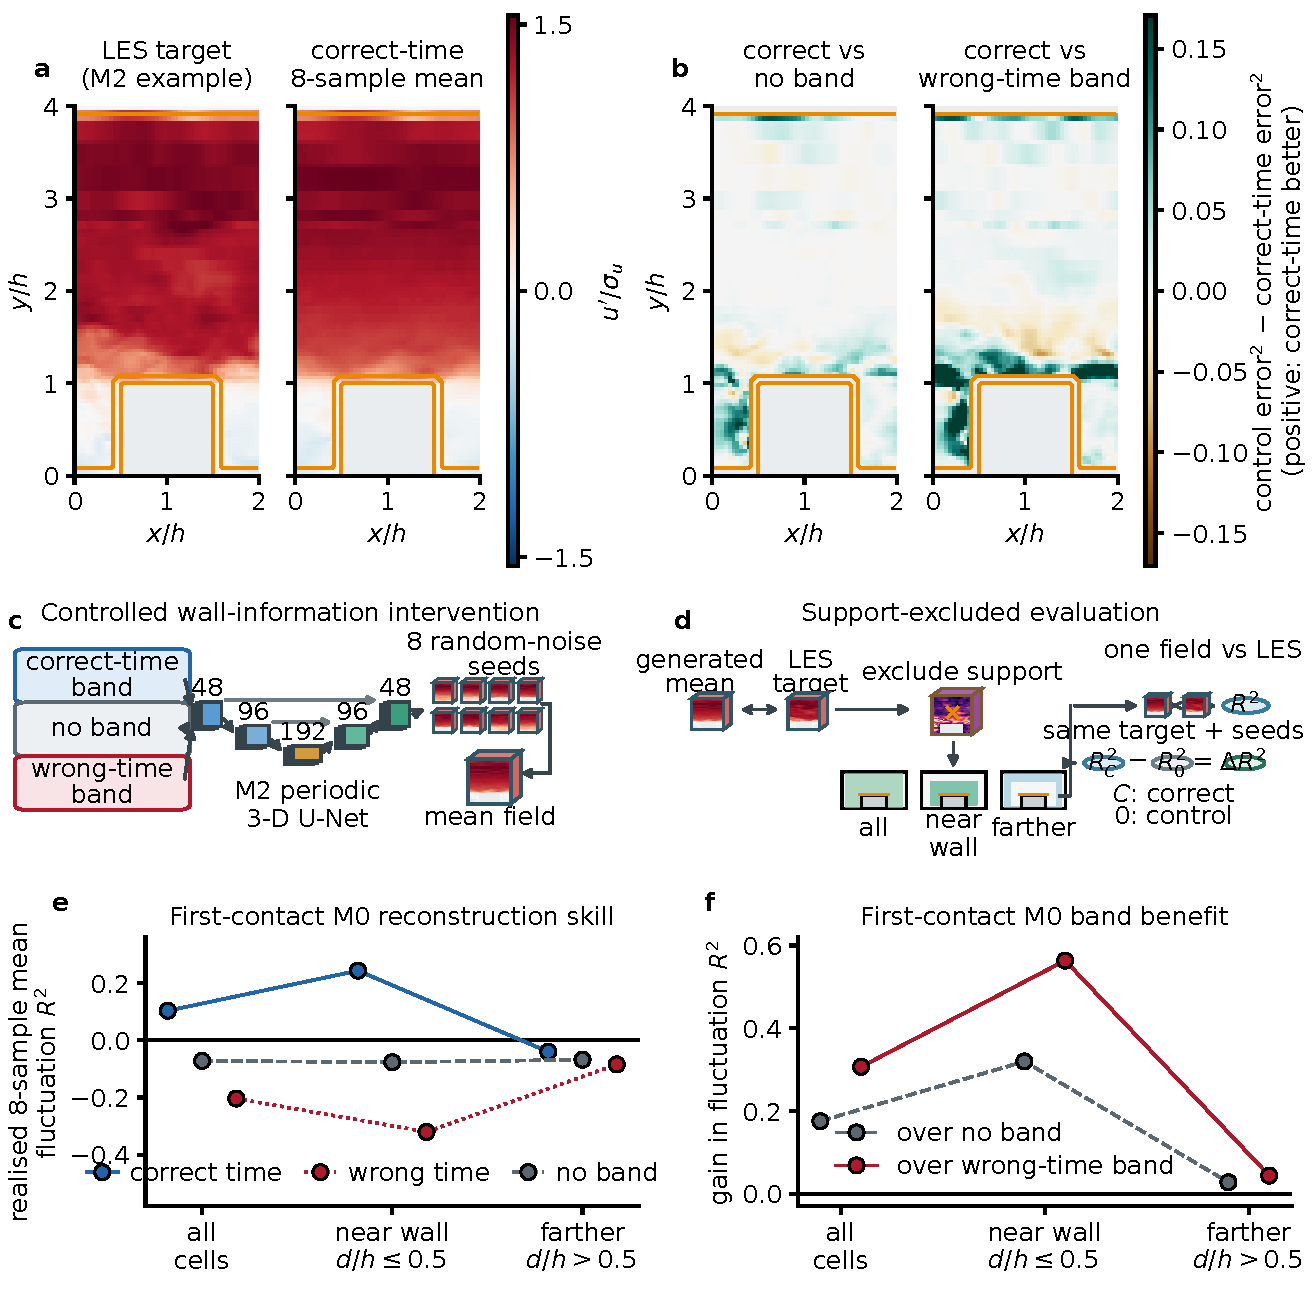
\includegraphics[width=\linewidth]{figures/fig3_propagation.pdf}
\caption{\textbf{Correct-time near-wall information acts chiefly near its supplied support.}
\textbf{a}, M2 mid-span LES target and eight-sample mean; orange marks supplied cells.
\textbf{b}, Local error reduction against no-band and wrong-time controls; green favours
correct time. \textbf{c}, Three matched arms traverse the frozen
3-D U-Net; larger cube, their eight-seed mean. \textbf{d},
All-cell, near-wall and farther masks; $R^2$ scores one arm,
$\Delta R^2$ a matched pair. Aligned, absent and far-time here score $0.120$, $-0.077$,
$-0.314$; near-wall aligned skill $0.284$. \textbf{e}, M0 field-to-LES $R^2$. \textbf{f},
Correct-time gain over controls. M0 points are terminal aggregates without replayable intervals,
but anchor interpretation as the only pre-contact comparison.}
\label{fig:point}
\end{figure}
\FloatBarrier

\emph{Post-selection distributional endpoint.} A registered farther-region energy-score
endpoint, frozen after M2 selection, favours the aligned arm over both controls ($0.522$
against $0.527$ and $0.548$)---a conditional post-selection sensitivity. \textbf{Its physical
corroboration is null}: both valid statistic families fail to beat both controls, and the
registered coverage family was withdrawn as invalid at eight members (Supplementary Note~4).

\subsection{An equilibrium velocity reconstruction destroys the interface}
\label{sec:interface}

A wall closure cannot supply a dense oracle velocity band; it supplies a signed two-component
wall traction. We first executed the standard adapter---expand that traction into a velocity band
through an equilibrium law and impose it. All arms use model M1, byte-identical to
Section~\ref{sec:first} in generator, targets, sampler noise and scoring masks; only the band
payload changes.

Two raster defects change how the published band should be read: supplied cells carrying no
information, and duplicates of scored cells. Restricting the band to the physical walls
removes both; the leak-free arm still improves on the absent branch by
$+0.102\,[0.093,0.109]$, so the computational ceiling accounts for about
42\% of the published $+0.174$ gain (Supplementary Note~3).

Against that matched ceiling the traction interface fails (Fig.~\ref{fig:interface}). The
target-velocity equilibrium inversion through the frozen lift scores $-0.117$ on the complete
volume, a change of $-0.032\,[-0.048,-0.021]$ relative to supplying nothing, and its transmission
ratio against the matched ceiling is $-0.320\,[-0.517,-0.194]$. The controls locate the failure: the traction is not information-free---the instantaneous
inversion beats the mean wall load and a far-time traction ($+0.199\,[0.162,0.239]$)---yet every
lifted arm sits below the absent branch (Fig.~\ref{fig:interface}b,c). The a-priori diagnostic explains why: the lifted
band reproduces the true band with fluctuation
$R^2=-0.109\pm0.185$, worse than the band's own mean, and the sampler clamps that error into the
field along the whole trajectory (Eq.~\eqref{eq:hard}).

This bounded negative falsifies only the composition tested. Two confounds live in the adapter,
not in the wall information: the lift is an equilibrium model of an instantaneous field, and
every lifted arm is outside the frozen generator's conditioning distribution. The next
subsections remove it.

\begin{figure}[t]
\centering
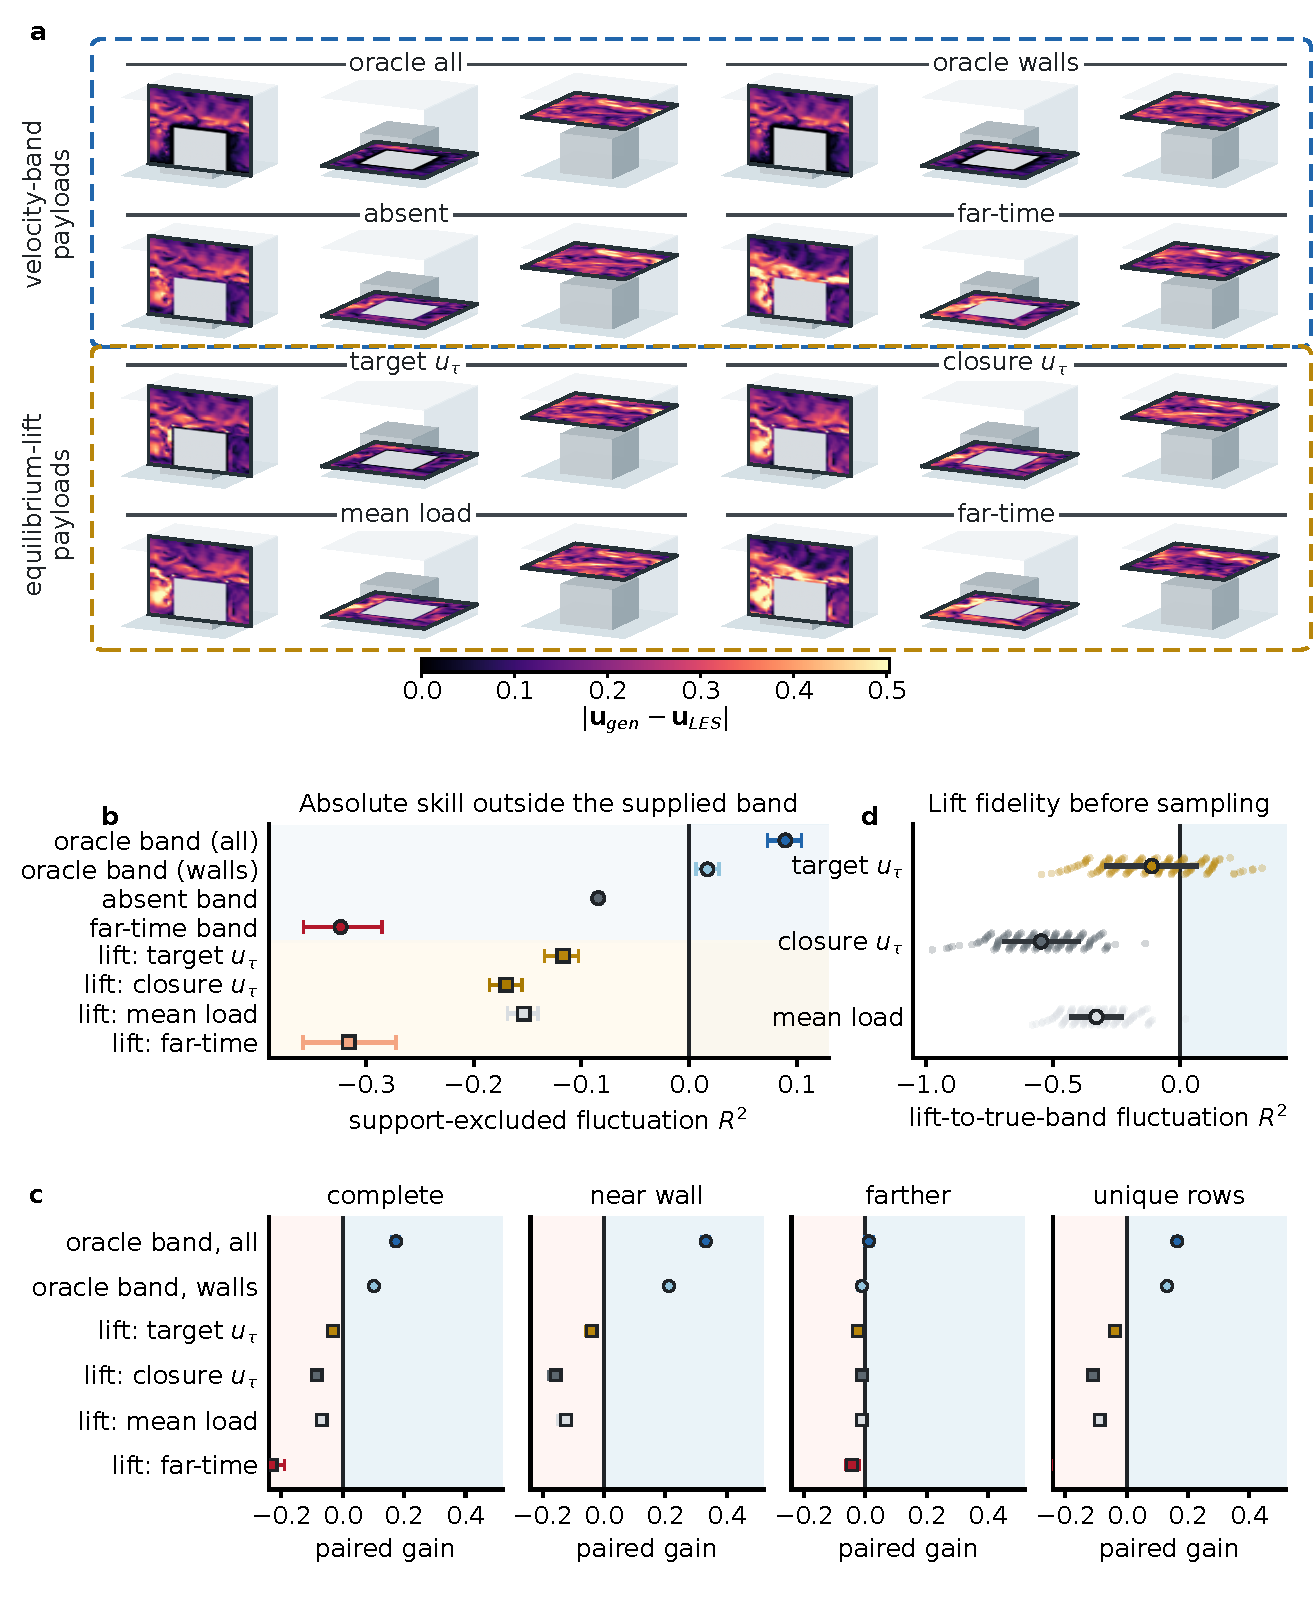
\includegraphics[width=\linewidth]{figures/fig6_interface.pdf}
\caption{\textbf{Frozen closure-to-generator interface.}
Only payload changes. \textbf{a}, Representative 3-D errors for eight payloads on mid-span,
near-wall and outer planes. \textbf{b}, Support-excluded $R^2$; a model-predicted traction with
no target-derived wall information (friction-velocity field correlated $0.782$ with the
inversion) scores $-0.085\,[-0.098,-0.073]$, and the instantaneous inversion beats the mean
wall load by $+0.037\,[0.021,0.054]$. \textbf{c}, Gain over absence by
region; whiskers in \textbf{b},\textbf{c} are conservative 95\% intervals. \textbf{d}, Target-wise
lift fidelity (mean $\pm$ s.d.). Oracle bands help; every lifted-traction arm underperforms
absence. This result covers only the frozen lift--generator composition, not general wall closures
or solver-coupled performance.}\label{fig:interface}
\end{figure}
\FloatBarrier

\subsection{A first-cell wall traction propagates without any velocity reconstruction}
\label{sec:direct}

Removing the adapter requires conditioning on the surface quantity itself. The tangential
projector annihilates the isotropic pressure term (Eq.~\eqref{eq:traction}), so a wall-on-fluid
traction is recoverable from the velocity record alone
(Eq.~\eqref{eq:nativetau}): a \emph{first-cell viscous traction} on the model raster, not the
native spectral-element derivative. Physical consistency checks ran before any arm was sampled
(Methods). Generators were then trained from scratch to condition directly on that traction---no velocity
reconstruction, no clamp---under a protocol frozen and hash-bound before the production run,
which discloses prior contact: a previously contacted record, not an untouched confirmation
($N_{\mathrm{eff}}=2.46$).

The contrast is positive in every scoring region (Fig.~\ref{fig:direct}). On the complete
unsupplied volume the first-cell traction improves support-excluded fluctuation $R^2$ by
$+0.074\,[0.070,0.078]$ over the absent-conditioning branch, with the same sign on all three
seeds (across-seed s.d. $7.52\times10^{-4}$); the near-wall gain is $+0.140\,[0.135,0.145]$,
decaying outward (Fig.~\ref{fig:direct}e). Against a matched ceiling---the oracle band on the same support, retrained identically
($+0.117\,[0.111,0.123]$)---the traction transmits $0.631\,[0.622,0.639]$.

The controls place the effect in the wall information, not the act of conditioning: the traction
arm beats a training-window mean load, a far-time, a shuffled and a sign-reversed traction by
$+0.077$ to $+0.204$ on the complete volume (Fig.~\ref{fig:direct}d). The shuffled and
sign-reversed fields are out-of-training inputs measuring sensitivity under distribution shift,
so the signed orientation is not by itself established as causal.
One contrast runs the other way: farther from the wall the sign-reversed arm beats the correct
one by $0.022\,[0.011,0.032]$.

Three limits bound this. The traction is read from the held-out target, so it measures what a
closure's output could transmit---closure accuracy is the question Sec.~\ref{sec:closurecomp}
answers. It is an invertible linear map of the first-cell tangential velocity
(Eq.~\eqref{eq:nativetau}), strictly less informative than the band, so a transmission ratio
below one is not by itself evidence of a lossy interface. And absolute skill remains negative
($-0.014$ against $-0.088$ for absence). 

\begin{figure}[!htbp]
\centering
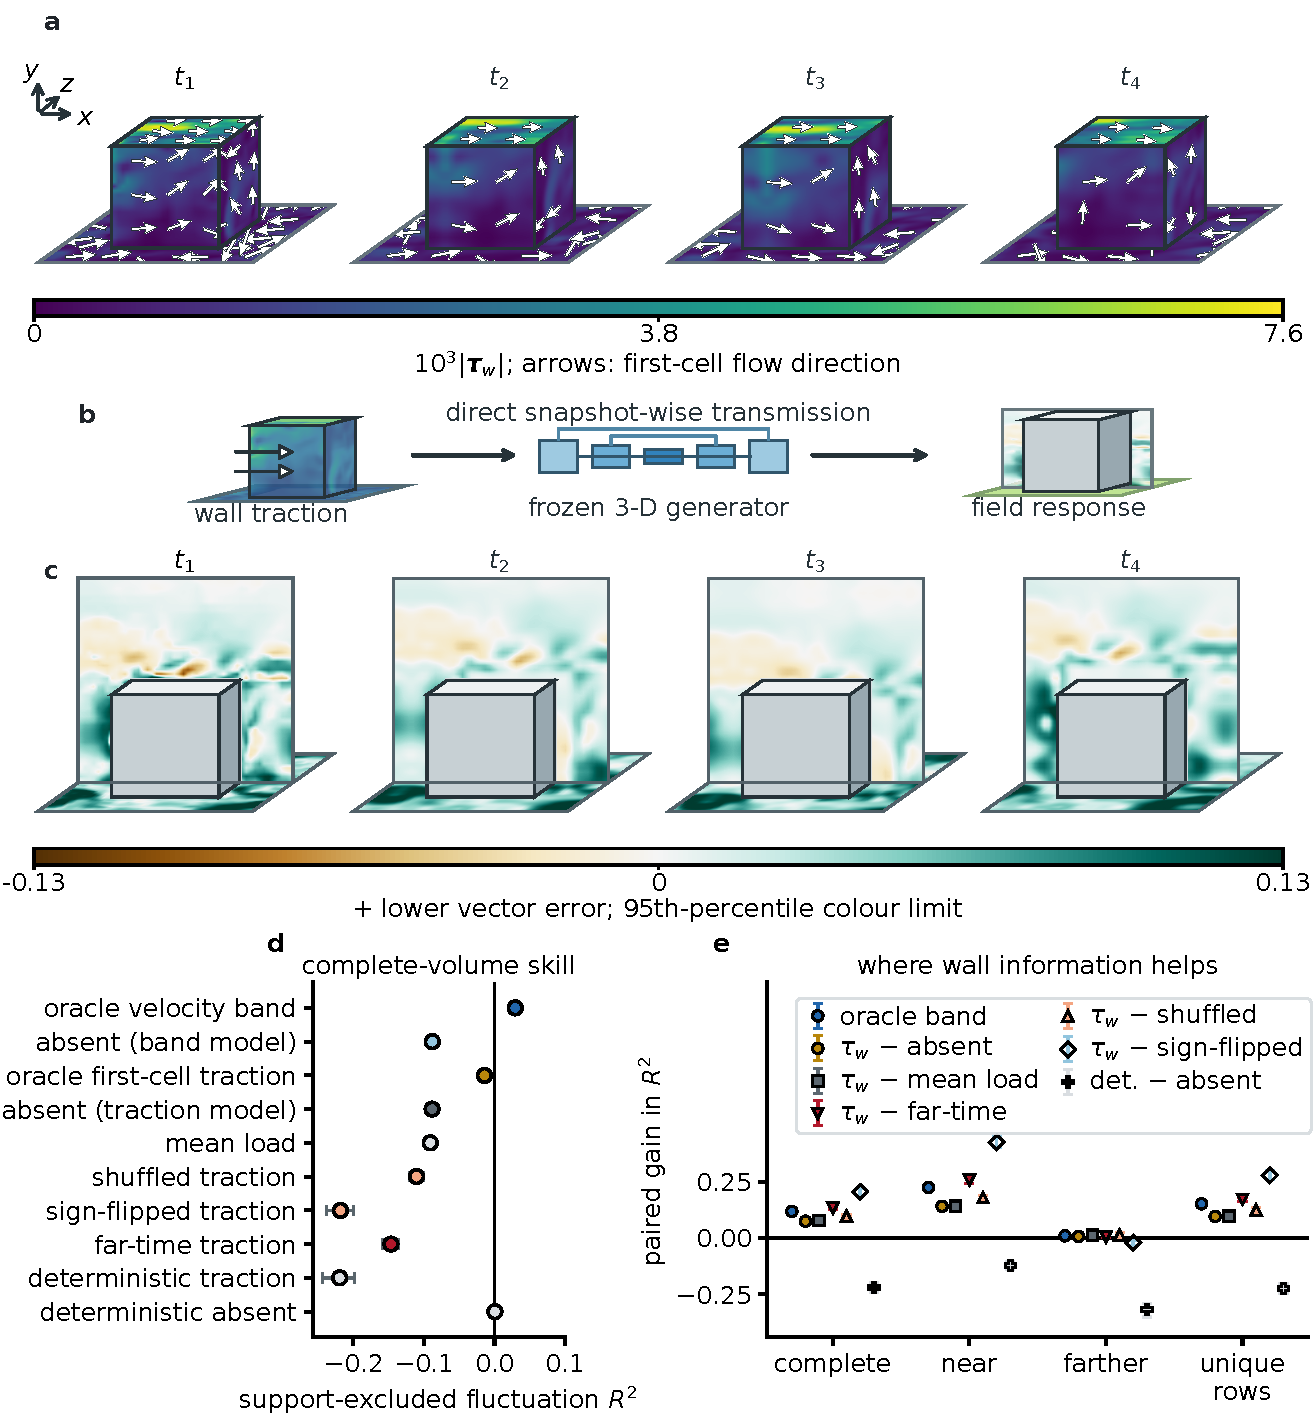
\includegraphics[width=\linewidth]{figures/fig7_direct_traction.pdf}
\caption{\textbf{Direct traction retains useful near-wall information.}
\textbf{a}, Wall-traction magnitude and first-cell flow direction at four illustrative instants.
\textbf{b}, Snapshot-wise transmission through the frozen 3-D generator.
\textbf{c}, Near-wall and midspan vector-error reduction (green indicates improvement).
\textbf{d}, Complete-volume skill across controls.
\textbf{e}, Paired gains across four regions; open markers denote out-of-training probes.
Intervals use conservative moving blocks. The traction is oracle---an invertible linear map
of the first-cell tangential velocity---and evaluated offline.}
\label{fig:direct}
\end{figure}
\FloatBarrier

\subsection{A closure that never sees the wall propagates into the field}
\label{sec:closurecomp}

Here we close the last map. A closure is fitted on the training window alone,
frozen by hash, and used to \emph{predict} held-out signed wall traction from matching-height
outer-flow state only---velocity at $2.5\Delta$ and
$4.5\Delta$ from each face, the wall-modelled-LES seam a coarse solver carries. It
never reads the wall-adjacent cell (Sec.~\ref{sec:closuremethodfit}), and its prediction is
all the generator receives. The score excludes every supplied cell \emph{and} every closure-read cell (8,040 more), with the
registered rule evaluated on 103 hash-bound held-out frames outside the direct-traction
experiment's index, prospectively unscored with prior contact recorded (Supplementary Note~1).

\emph{The closure.} On those frames the closure predicts the first-cell traction with
zero-traction-reference skill $0.540$ and mean direction cosine $0.746$, against $0.413$ for the
classical equilibrium wall model it contains as the case $a=\theta=0$
(Fig.~\ref{fig:closurecomp}e,f). The statistic normalises mean squared error (MSE) by the training-window root-mean-square rather than centring it
(both conventions in Sec.~\ref{sec:reachgated}); fit, validation and held-out scores are
$0.553$, $0.539$ and $0.540$, consistent with a 5,426-parameter correction that has not
overfitted.

\emph{The composition.} Conditioning the generator on that predicted traction improves
source-excluded fluctuation $R^2$ by $+0.061\,[0.057,0.064]$ over the absent-conditioning branch
of the same network, with the same sign on all three seeds and a crossed seed$\times$block
interval of $[0.055,0.065]$ that also excludes zero. The gain is $+0.118\,[0.112,0.124]$ near the
wall and positive under all seeds farther out (Fig.~\ref{fig:closurecomp}h).
All five registered clauses pass, computed mechanically from the released decision-rule record.
This is the paper's central claim: a wall quantity a closure actually produces---not one read
from the answer---propagates into the surrounding field.

\emph{Controls.} The decisive control is a far-time traction---a genuine traction of the wrong
instant, and a training class of this generator, so no distribution-shift confound. It is
\emph{worse than supplying nothing} ($-0.043\,[-0.053,-0.030]$), and the closure beats it by
$+0.104\,[0.092,0.114]$: wall information helps only at the right instant. A mean-load, a
shuffled and a sign-reversed traction are also below absence
(Fig.~\ref{fig:closurecomp}h).

\emph{Where the gain comes from.} At matched input information the learned non-equilibrium
correction is worth $+0.013\,[0.003,0.021]$ over the pure equilibrium closure, and the closure
arm exceeds the oracle traction arm by $+0.013\,[0.003,0.021]$---not prediction beating truth,
since the arms carry \emph{different} information and a closure's matching-height view is at
least as useful for propagation as an exact wall derivative. Complete-volume absolute skill
nevertheless remains negative for every arm ($-0.028$ closure against $-0.088$ absence, $-0.041$
oracle, $-0.131$ far-time).

\emph{Distributional validation.} The closure arm has the lowest continuous ranked probability
score (CRPS), per-cell energy score
and rank-histogram reliability deviation of any arm at every ensemble size
(Fig.~\ref{fig:closurecomp}d): the improvement is distributional, not an artefact of averaging.

\emph{A bounded engineering consequence.} The streamwise viscous wall force inferred from the
generated field---an offline reconstructed first-cell diagnostic excluding pressure and form
drag, not the traction a solver would consume---falls in relative RMSE from $0.099$ to $0.061$
with the closure, its correlation with the true load rising from $-0.178$ to $+0.741$
(Fig.~\ref{fig:closurecomp}g). The equilibrium closure is \emph{worse} than absence here despite
a similar field-$R^2$ gain: the learned correction matters far more for wall load than for
volume-averaged skill.

\emph{Transfer and non-regression.} The frozen generator of Sec.~\ref{sec:direct}, reused
byte-for-byte, gains $+0.036\,[0.024,0.046]$ from the predicted traction against $+0.052$ for
the oracle traction it was trained on---about seven-tenths, the expected cost of feeding a
predicted signal to a model trained on measured ones. Replaying the frozen checkpoints on that
experiment's exact frames reproduces its published values within the frozen $0.005$ identity
tolerance, and all eight prospectively frozen tolerances pass.

\begin{figure}[!htbp]
\centering
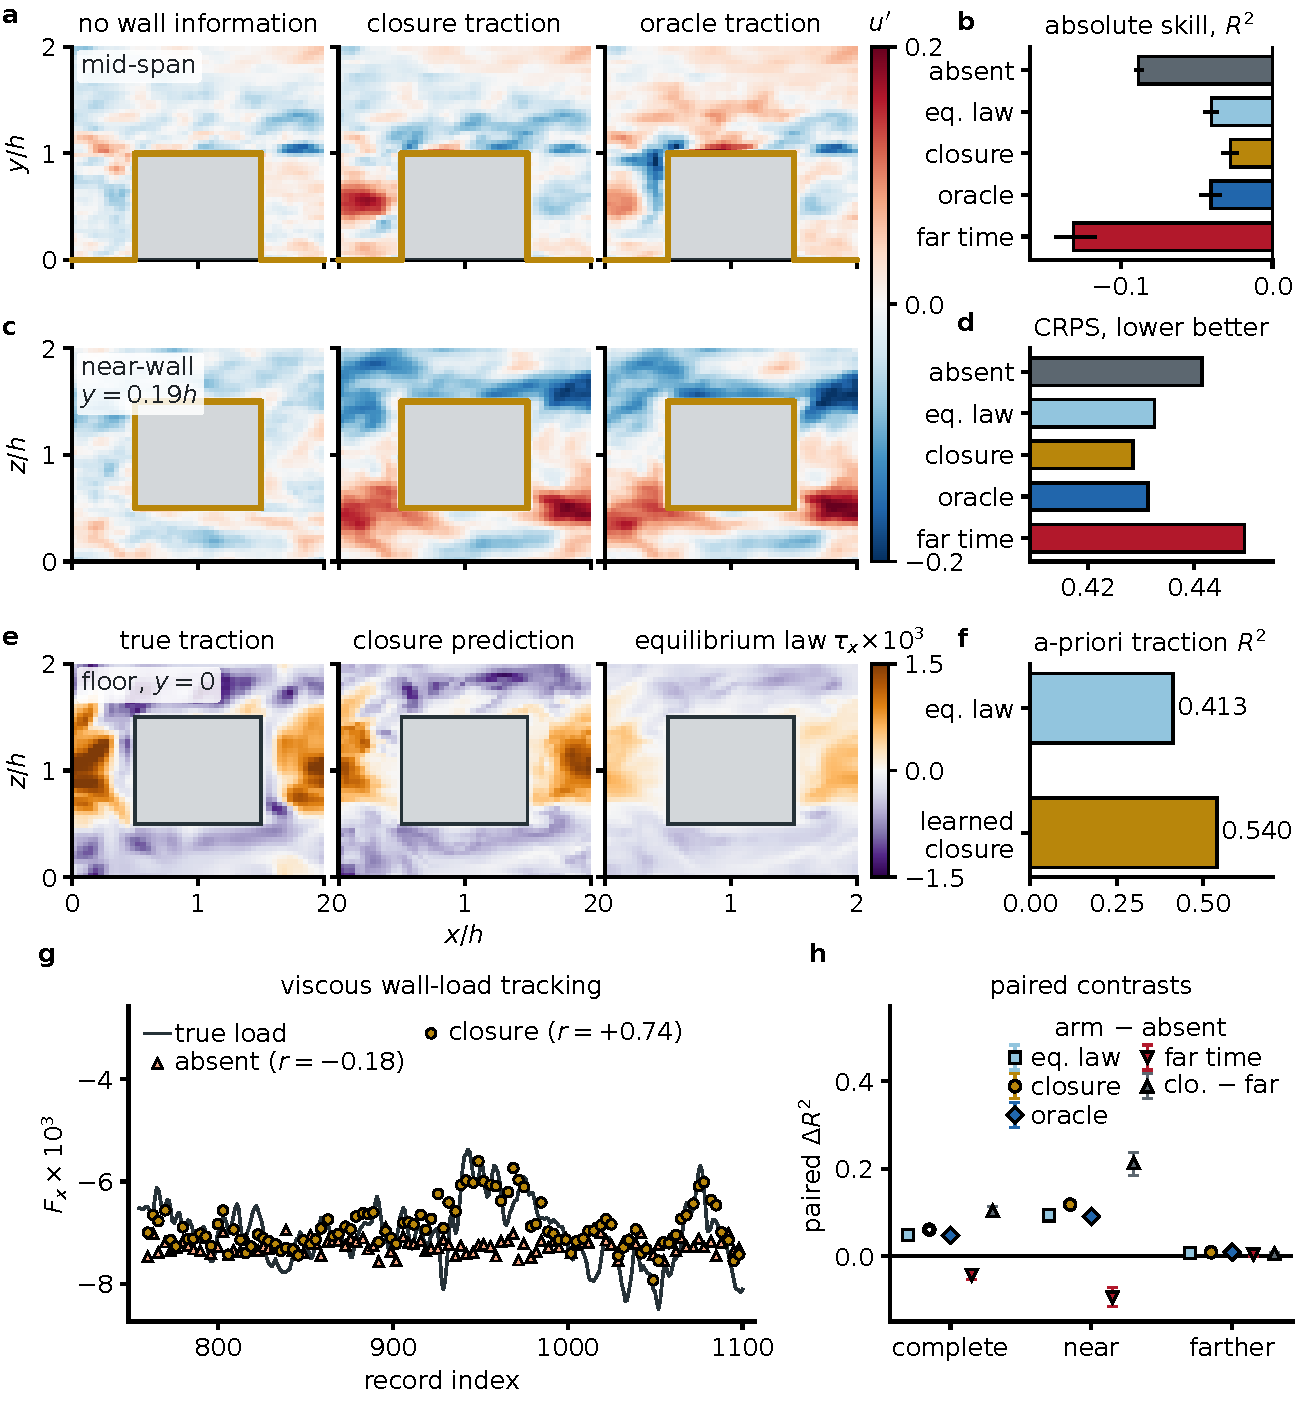
\includegraphics[width=\linewidth]{figures/fig8_closure_composition.pdf}
\caption{\textbf{A physics-grounded wall closure supplies traction that propagates through the
generative model.} \textbf{a},\textbf{c}, Posterior-mean streamwise fluctuation of held-out
record 760, mid-span and near-wall ($y=0.19h$): absent, closure, oracle traction;
gold marks traction-carrying walls. \textbf{b},\textbf{d}, Absolute source-excluded skill
(every arm negative) and CRPS; closure-arm energy score $0.922$ against $0.948$
(absent), reliability deviation $0.146$ against $0.165$. \textbf{e}, Floor
traction: true, closure-predicted, equilibrium. \textbf{f}, A-priori traction skill.
\textbf{g}, Implied viscous wall force vs true load (oracle: relative RMSE $0.035$,
correlation $+0.927$; equilibrium $0.160$, bias $+0.147$). \textbf{h}, Registered paired
contrasts; open circles, seeds. Scored on 103 prospectively unscored frames, outside every
supplied and closure-read cell; offline.}\label{fig:closurecomp}
\end{figure}
\FloatBarrier

\subsection{The interface transmits on a separating flow}\label{sec:generality}

The cube wall is geometrically pinned. To ask whether the composition survives a wall whose
stress is set by the flow, the identical protocol was re-executed on the \emph{separating
periodic-hill} flow \cite{frohlich2005highly,breuer2009hill,xiao2020hills} at $Re_h=2800$ in both
generative families and at two rasters, together with the cube under a \emph{denoising-diffusion}
generator \cite{ho2020ddpm}. The hill wall is smooth and curved, with
pressure-gradient-induced separation---the regime where equilibrium wall models fail
(Fig.~\ref{fig:reachgated}a--c). It is a 2-D $(u,v)$ corpus with no spanwise dynamics.

Two properties of the protocol travel to any wall-to-field study.
\emph{The evaluation unit is the physical time, not the stored array}: this corpus stores three
spanwise planes per physical time, correlated up to $0.996$, so scoring groups planes by physical
time and separates training from scoring by $110$ of them. A flattened array-index split instead
hands each test frame its own same-time twins during training, inflating $R^2_{\rm fluct}$ by
$0.839$ (Supplementary Note~10). And \emph{a unit must show it can detect wall information before
it may adjudicate the interface}: no conclusion is drawn unless conditioning on true near-wall
information improves reconstruction with an interval excluding zero. A contact audit
shows no physical time of this record is untouched by earlier analyses, ours included.

The record passes that control in the diffusion family, and so does the method. Supplying the
traction \emph{directly}---the surface quantity the generator was trained to read---the record's
own exact direct-numerical-simulation (DNS) traction improves source-excluded fluctuation $R^2$
by $+0.058\,[+0.009,+0.107]$, and the traction predicted by the frozen closure, which never reads
a wall-adjacent cell, improves it by $+0.062\,[+0.017,+0.106]$, both proper scores agreeing
(CRPS $-0.0124\,[-0.0188,-0.0056]$; energy score $-0.0172\,[-0.0268,-0.0076]$). Two paired
contrasts say what that gain is made of: the closure arm is not resolved from the exact
traction ($+0.004\,[-0.007,+0.017]$)---no advantage of the wall truth over the fitted closure
is detected here; and the traction signal is \emph{read} rather than merely present, the
closure arm beating the same traction from a wrong instant by $+0.045\,[+0.001,+0.086]$ over the
volume and $+0.101\,[+0.017,+0.170]$ near the wall, where wrong-instant information falls
\emph{below} supplying nothing.

The bounds matter as much. The near-wall interval for the closure arm alone crosses zero
($+0.063\,[-0.022,+0.152]$), and the arm is separated from neither a magnitude-matched scrambled
traction ($+0.026\,[-0.021,+0.067]$) nor the equilibrium law ($+0.011\,[-0.015,+0.031]$), so
specificity holds against wrong timing but is unresolved against wrong spatial pattern; absolute
skill stays negative for every arm. With $370$ scored times against a measured integral time of
$112.3$, $N_{\rm eff}\simeq3.3$: every hill interval here, favourable and adverse alike, is
indicative rather than precise, and the hill is not part of this paper's headline claim.

How the traction is presented decides whether it transmits. Expanding it first into a near-wall
velocity band through the closure's Reichardt profile does \emph{not} clear zero at either raster
($+0.038\,[-0.017,+0.091]$ at $64\times192$; $+0.059\,[-0.011,+0.122]$ at $96\times288$), despite
that lifted band reproducing the true band velocities at $R^2=0.871$ and $0.915$ and the
equilibrium lift matching it to three decimals: fidelity in the lifted representation is not
sufficient. The oracle band arm, which \emph{is} the record's exact band rather than a lift, does
pass at both rasters ($+0.057\,[+0.011,+0.107]$ and $+0.079\,[+0.027,+0.131]$;
Fig.~\ref{fig:reachgated}f); its scrambled control is itself weakly positive over the whole
volume ($+0.018$), so part of any whole-field gain is non-specific, but near the wall that
vanishes and wrong information falls below absence.

At the wall the record is positive in both families. The closure predicts wall traction on the
time-disjoint unit with $R^2=0.757$, against $0.557$ for the equilibrium law it contains
(Fig.~\ref{fig:reachgated}d), and conditioning on it improves the reconstructed wall force
($0.036\to0.542$ and $-0.104\to0.445$ in correlation)---an offline reconstructed first-cell
viscous-force diagnostic excluding pressure and form drag. The wall quantity is recovered even
where the outer field is not: the near-wall/whole-field dissociation volume-averaged objectives
conceal. The flow-matching cell fails the same positive
control at both rasters, so by the standing rule it cannot adjudicate the interface in either
direction; that arm and its failed repair are treated in the
Discussion. Every registered contrast, sampler, raster and control is
tabulated in Supplementary Note~10, with two further checks that fail their preregistered
criteria, the withdrawn composition attempts and the custody audit that forced refitting the
closure on the cube record (Supplementary Notes~6--8).


\subsection{A re-test on a record that passes the control shows the interface transmits, and how
far}
\label{sec:reachgated}

To decide the whole-field question on a unit with demonstrated detectability, we re-executed the
frozen closure$\rightarrow$traction$\rightarrow$generator composition on the wall-resolved cube
record with three changes fixed before any outcome existed (Supplementary Note~11): the split is
\emph{reversed in time}, everything refitted from scratch on late frames and scored on a
never-tested $25$-frame window $132$ frames from training; both families are trained at an
identical budget with one frozen conditioning mixture including the oracle band, so band and
traction arms are compared \emph{within one propagator}; and the near-wall region $d\le0.5$ is
co-primary with the whole field. That region is outcome-informed, hence evaluated on a fresh unit.

The positive control passes in both families ($+0.130\,[0.115,0.145]$ and
$+0.029\,[0.026,0.032]$; Fig.~\ref{fig:reachgated}g), and so does the interface. Conditioning on
traction predicted by a closure that never reads a wall-adjacent cell raises near-wall
fluctuation $R^2$ from $-0.098$ to $+0.005$, a gain of $+0.103\,[0.091,0.115]$
(Fig.~\ref{fig:reachgated}h)---the first arm here with positive absolute skill, recovering
$79\%$ of the DNS-band ceiling in the same propagator. The matched controls
separate cleanly: a spatially shuffled traction of identical support and magnitude multiset
scores $-0.128$ and a wrong-instant field $-0.164$, both \emph{worse} than supplying
nothing---the generator reads arrangement and instant, not the presence of a channel.

The effect has the wall-normal structure a boundary condition must have
(Fig.~\ref{fig:reachgated}i): in nested shells the same frozen contrast decays monotonically from
$+0.266\,[0.221,0.317]$ at $d\le0.15$ to $+0.006\,[0.004,0.008]$ beyond $d>0.5$, the nearest
scorable shell reaching $R^2=+0.149$ absolute against $-0.117$ unsupplied. The gain is $5.0$ times
larger beside the wall than in the whole-field average and $46$ times larger than in the outer
region, while the whole-field gain, $+0.053\,[0.046,0.063]$, replicates the registered $+0.061$
of Sec.~\ref{sec:closurecomp} on an independent, reversed-time unit.

Because the decisive window has $N_{\rm eff}=1.21$, the claim does not rest on the interval:
the paired per-frame difference is positive in $25$ of $25$ held-out frames for both
flow-matching seeds (minimum $+0.042$; diffusion $25/25$ and $24/25$;
Fig.~\ref{fig:reachgated}j).

The engineering-facing consequence is the reconstructed first-cell \emph{viscous} wall
force, an offline surrogate excluding pressure and form drag: closure conditioning moves its
correlation with the true load from $-0.14$ to $+0.51$ (Fig.~\ref{fig:reachgated}k;
Supplementary Note~11). One adverse detail is reported: the shuffled control attains a
\emph{higher} wall-force correlation ($+0.61$), mechanically, since permuting whole traction
vectors leaves the integrated force invariant---this integral cannot discriminate arrangement
while the field endpoint does.

Two limits are registered rather than argued away. The rule frozen before this run returns
\textbf{fail} on one clause---the diffusion family's \emph{absolute} unconditional skill,
$-0.53$, does not reach the inherited $-0.14$ floor, even though its interface delta is positive
and interval-separated; a development sweep locates that in the family's posterior mean rather
than in the interface, and the threshold was not adjusted after the outcome. And while the
closure captures the held-out traction pattern better than the equilibrium law
(Fig.~\ref{fig:reachgated}e), the instantaneous departure from the held-out mean traction remains
largely unpredicted (Supplementary Note~11).

As in Sec.~\ref{sec:closurecomp} the closure arm slightly exceeds the \emph{oracle traction} arm
($+0.005$ versus $-0.015$); the oracle band remains above both.

\begin{figure}[t]
\centering
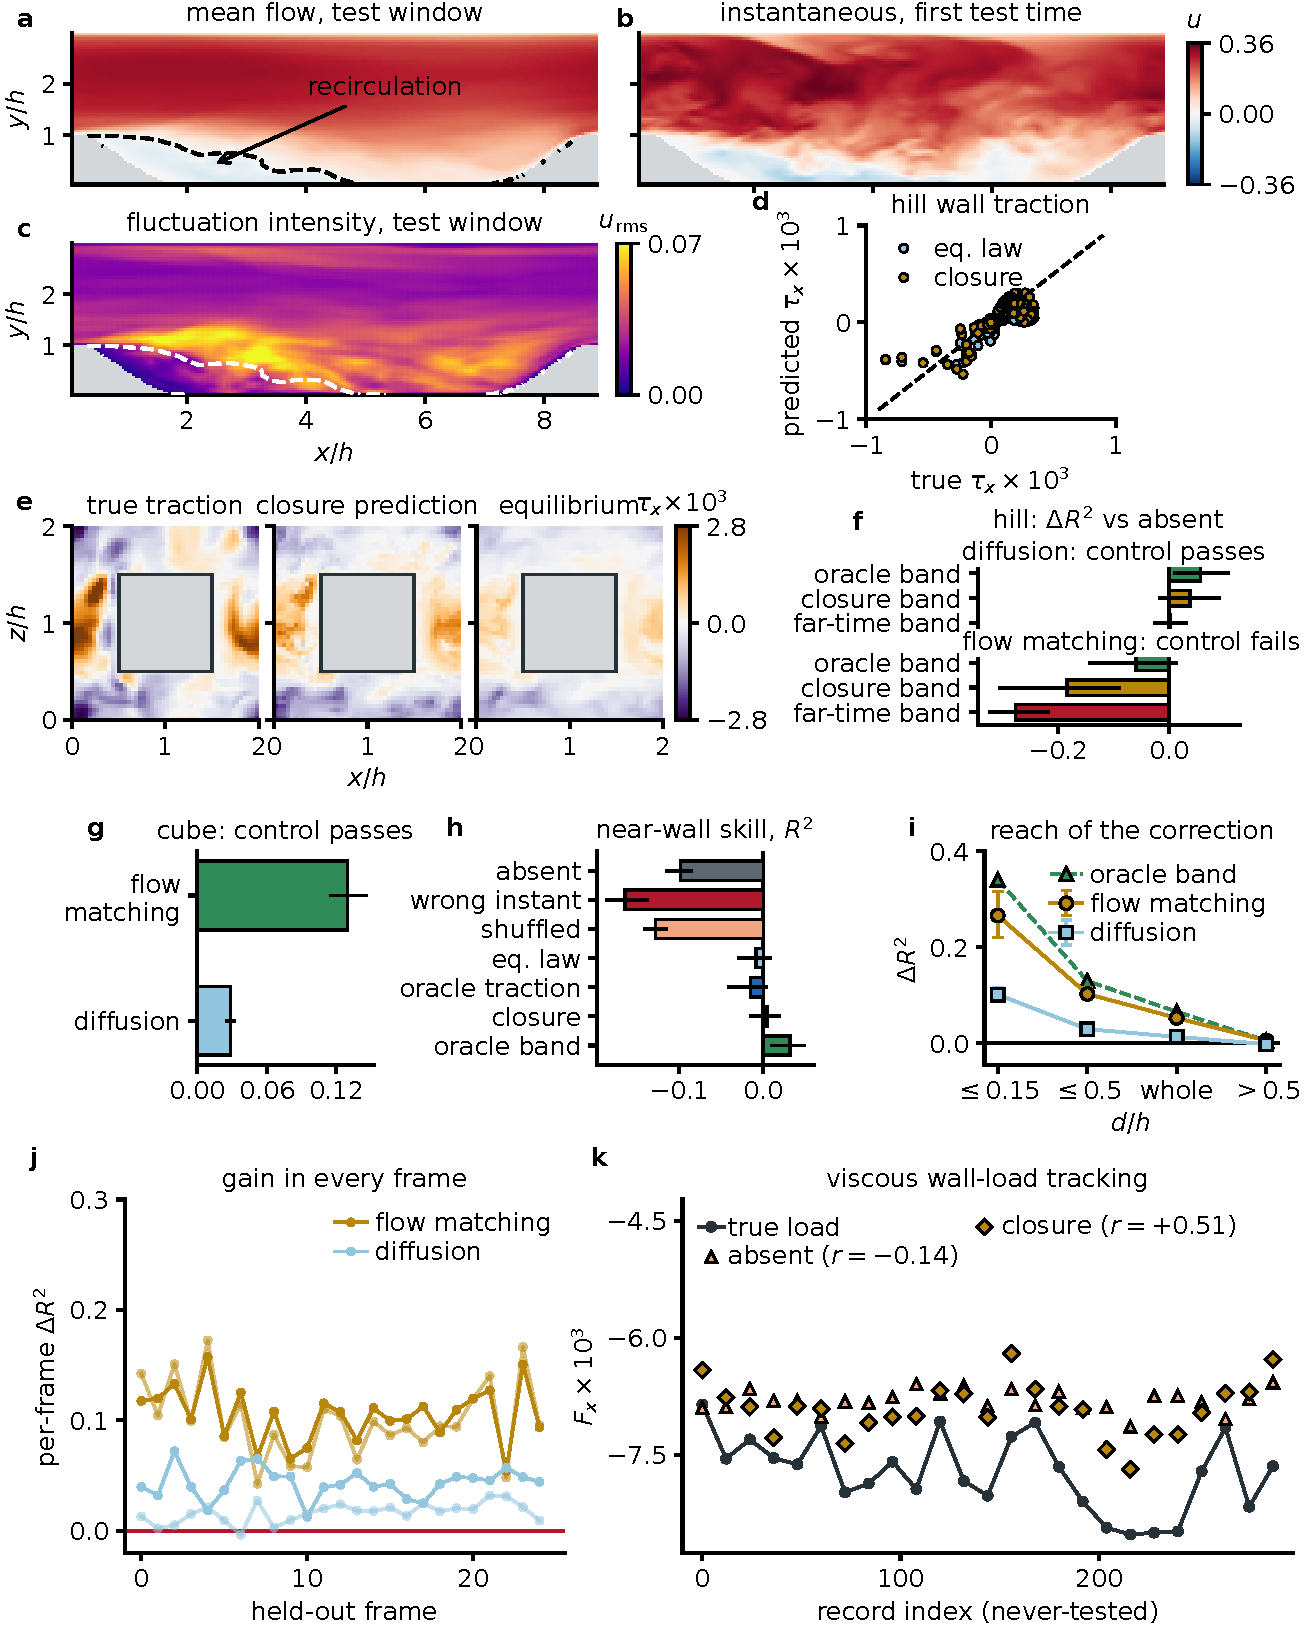
\includegraphics[width=\linewidth]{figures/fig11_reachgated_composition.pdf}
\caption{\textbf{A prospectively frozen oracle positive control decides which cells may
adjudicate the interface.} \textbf{a}--\textbf{c}, Separating hill: test-window mean flow
(dashed, $\bar u=0$), an instantaneous frame, shear-layer fluctuation intensity.
\textbf{d},\textbf{e}, Held-out traction on the separating wall and a never-tested cube frame.
\textbf{f}, Each band arm's paired contrast against its own absent branch at $64\times192$; the
label gives that family's \emph{positive-control} verdict, not a verdict on the closure arm. The
flow-matching failure survives a stochastic sampler and a finer raster (Supplementary Note~10).
\textbf{g},
Positive control on the reversed-time cube. \textbf{h}--\textbf{k}, Near-wall ladder; reach
against ceiling; per-frame gain; viscous wall-load tracking. All endpoints offline.}
\label{fig:reachgated}
\end{figure}
\FloatBarrier

\subsection{A single-slot channel experiment measures what transmitted traction is worth}
\label{sec:slot}

Earlier generators saw named wall-signal classes during training. A prospectively registered
single-slot experiment on a second, wall-resolved
record---the smooth-wall channel of the public CoNFiLD release at
$Re_\tau=184$---removes that asymmetry. The generator is trained on exactly one
traction-carrying condition, the record's own signed traction under a variance-preserving
fidelity ladder, so every wall model enters the same slot with zero generator-side training
exposure. A sublayer projection makes the generated wall gradient equal the supplied traction
identically, the conditioning rows ($y^+\le3.2$) are machine-verified absent from every scored
cell, and the never-scored 46-frame window was contacted only after a two-stage preregistration
froze every decision rule, control and margin (Methods).

On that window the record's own traction---the training modality---raises support-excluded
fluctuation $R^2$ by $+0.165$ ($t=204.7$ against a simulation-calibrated critical value of
$4.5$), and four graded reference arms trace a strictly monotone response ($+0.104$ to $+0.153$ at
fidelities $0.082$--$0.797$; Spearman $1.0$; Fig.~\ref{fig:slot}g). The closure,
reading only two matching-height velocity lines and never any cell below $y^+\approx29$, gains
$+0.120$ over supplying nothing ($t=36.5$; every block,
seed, wall and frame individually positive), with \emph{positive} absolute skill ($+0.030$
and $+0.035$ by seed against $-0.091$ and $-0.083$) and the wall-normal structure a boundary
condition must have: $+0.328$ in the buffer layer, $+0.066$ at $30<y^+\le100$, $+0.0001$
beyond (Fig.~\ref{fig:slot}f).

Attribution is read from the registered controls. The closure stays below the exact-traction
reference ($-0.045$) and, at its own fidelity ($0.023$), sits $+0.016$ above the lowest rung,
inside the frozen $0.02$ margin. The data-only regressor, with better fidelity ($0.083$), gains
more ($+0.131$): scalar fidelity orders, but does not alone predict, downstream gain, and the
ladder is a within-family sensitivity, not a universal law. Wrong wall information does not
merely fail: a wrong-instant traction scores $-0.060$ \emph{below} supplying nothing (closure
better by $+0.180$), a spanwise-shuffled traction is beaten by $+0.144$ and the equilibrium law
by $+0.044$. The mechanically applied rule concludes the interface transmits traction information
within the frozen margins.

The registered engineering endpoint improves: in the buffer band, outside every conditioning and
read row, the tracking error of the spanwise-averaged turbulent shear
$\langle u'v'\rangle$ falls by $26\%$ with the closure ($0.191\to0.141\,u_\tau^2$; $t=8.61$)
and $37\%$ with the exact traction. CRPS improves in the same direction ($t=98.7$; secondary);
the pooled rank histograms \cite{hamill2001interpretation} are U-shaped for every arm, an
underdispersion reported descriptively. The diffusion family
reproduces the primary contrast with both seeds positive ($+0.106$).

\begin{figure}[t]
\centering
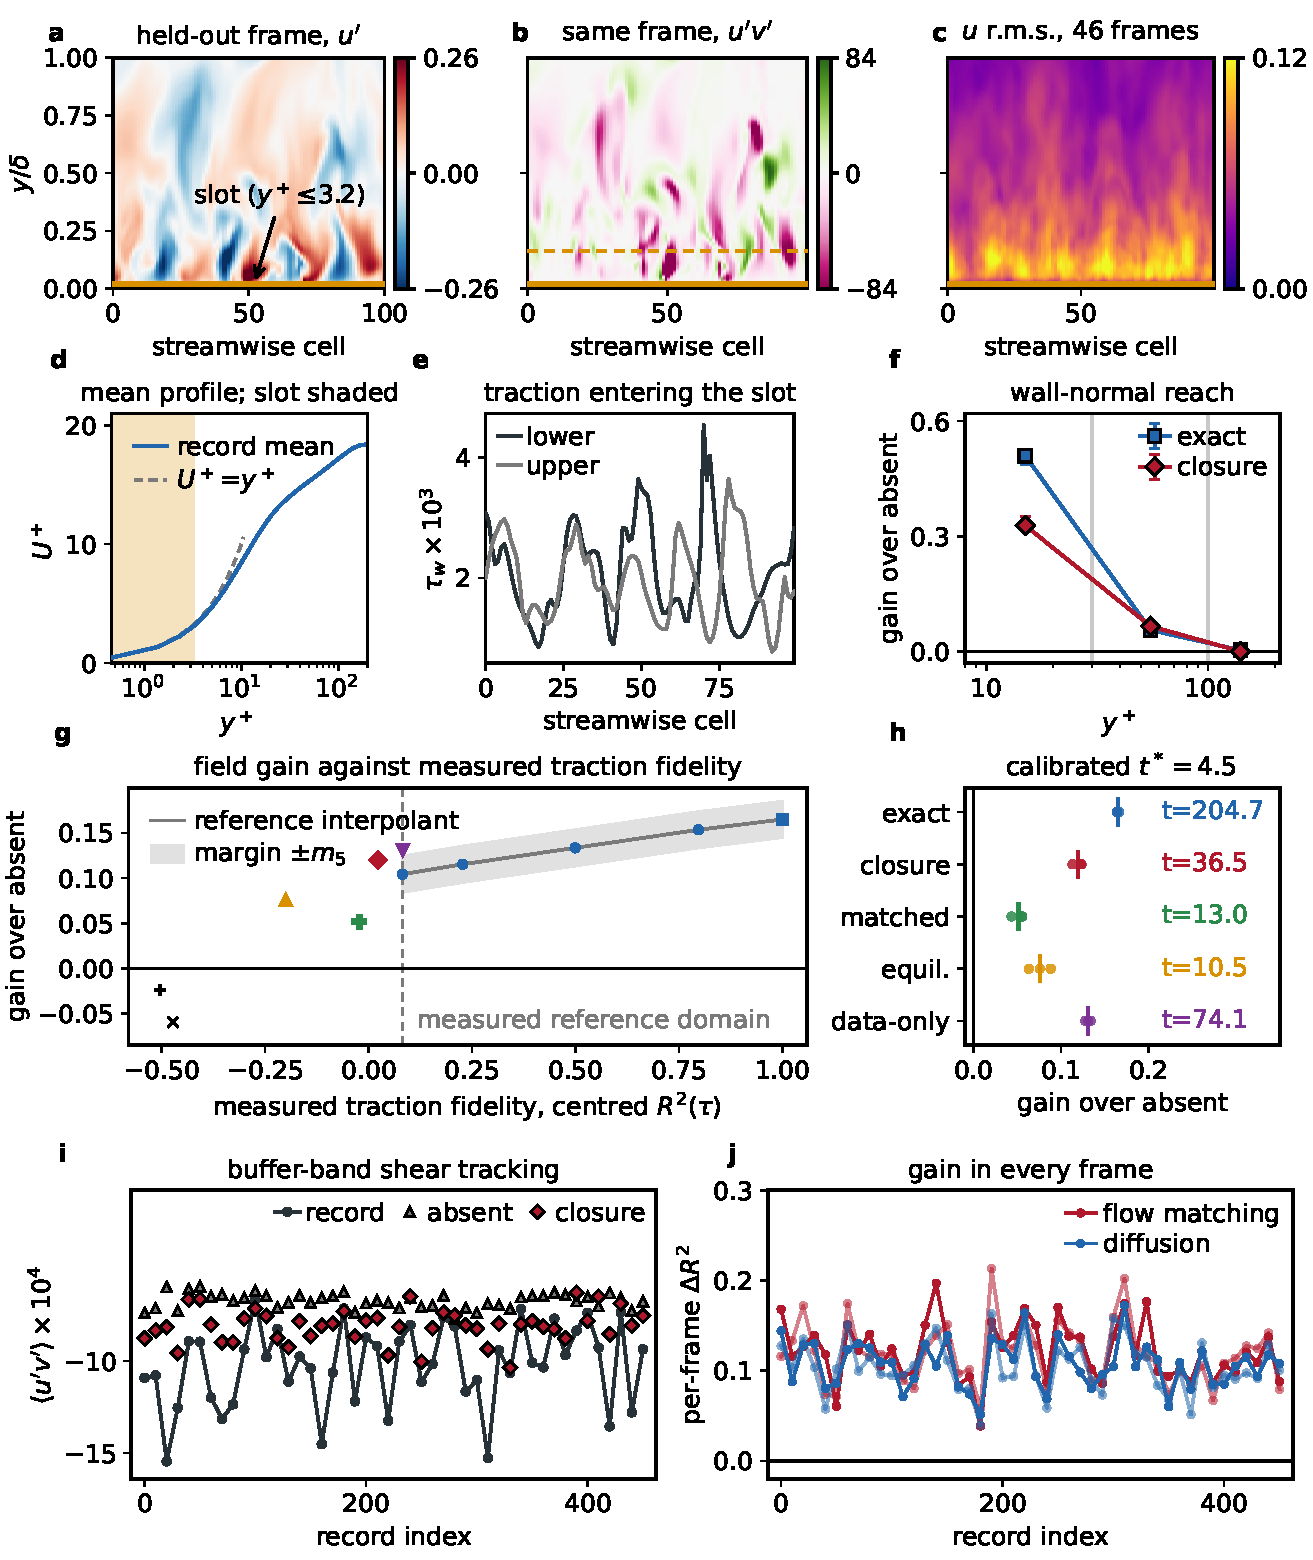
\includegraphics[width=\linewidth]{figures/fig14_slot_interface.pdf}
\caption{\textbf{A single-slot channel experiment: transmitted traction information improves
the generated field.} \textbf{a}--\textbf{c}, The wall-resolved record: a held-out frame's
$u'$, its $u'v'$ (buffer band dashed), and $u$ r.m.s.\ over 46 frames; gold marks the
conditioning slot ($y^+\leq3.2$). \textbf{d},\textbf{e}, Mean profile in wall units; slot
traction on both walls. \textbf{f}, Wall-normal reach. \textbf{g}, Field gain against
measured traction fidelity; the lowest rung ($r=0.55$) still correlates
structurally with the true traction. \textbf{h}, Block inference at the calibrated
$t^\ast=4.5$. \textbf{i}, Reconstructed buffer-band turbulent shear tracking:
per-frame error $3.84\times10^{-4}$ (absent), $2.83\times10^{-4}$ (closure),
$2.40\times10^{-4}$ (exact traction). \textbf{j},
Per-frame gain; every frame, seed and family positive.}
\label{fig:slot}
\end{figure}
\FloatBarrier

\section{Discussion}\label{sec:discussion}

This paper evaluates one integrated system end to end: a physics-grounded wall closure connected
to a conditional generator.
Reading matching-height flow state, the closure predicts held-out traction better than its
equilibrium law ($0.540$ against $0.413$); supplying it improves source-excluded fluctuation
$R^2$ by $+0.061\,[0.057,0.064]$ under a pre-fixed rule. The unit was prospectively unscored,
not independent.

On the separating hill, the diffusion positive control passes and closure traction gains
$+0.062\,[+0.017,+0.106]$, not resolved from exact traction and better than wrong-time
traction. Roughly three effective samples make this indicative rather than precise.

One preregistered arm was adverse: flow matching fails its positive control and cannot adjudicate
the interface. We tested the obvious under-dispersion explanation prospectively with a stochastic
sampler on byte-identical weights; dispersion improved while the control failed \emph{more}
clearly. A model-family difference in how sparse wall information is used remains plausible, but
no mechanism is established. Ensemble dispersion is therefore reported as a diagnostic, never an
acceptance criterion (Supplementary Note~10).

Two properties make the cube number interpretable: its decisive
control is a real traction of the wrong instant, scoring worse than supplying nothing, so the
model is rewarded for \emph{this instant's} wall state; and the gain is distributional, the
closure arm best on every proper score at every ensemble size.

The practical reading is specific: expanding wall stress into an equilibrium-law velocity band
and clamping it fails, whereas the same quantity transmits through conditioning trained to read
it. The instantaneous field a generator needs is not the field an equilibrium law describes.

The limits are stated once, each marking where the evidence ends and the next study begins. The
composition is established offline and a priori, never inside a time-evolving solver.
Complete-volume absolute skill on the cube record stays negative for every
arm ($-0.028$ closure against $-0.088$ absence)---wall information moves the field towards the
target without yet making it accurate---while the re-test's near-wall region and the channel
record reach positive absolute skill. All three records carry few effective independent events,
so every interval is conditional on them---the price of difficult engineering records over
abundant homogeneous ones. The farther-from-wall gain, $+0.009\,[0.003,0.016]$, is
the honest measure of reach; the out-of-training probes are sensitivity checks, not causal
controls; and the fitted target is a first-cell viscous traction on the model raster, not the
native spectral-element gradient. The closure reads its matching heights at fixed multiples of
the local cell size, $2.5\Delta$ and $4.5\Delta$---the seam a wall-modelled solver carries---so
the multiples and the mesh setting $\Delta$ are parameters of the interface itself, and the
natural first task for a deployment study is charting the gain's response to coarser rasters and
different seams. The same standard then extends to the regimes most likely to strain the
interface: unresolved near-wall bands, spanwise three-dimensional near-wall structure, rough
walls and Reynolds numbers far above these records, where the wall's far-field footprint
grows.

The supportable engineering consequence is offline and specific: the implied streamwise viscous
wall-force error falls by almost two-fifths with the closure, while the equilibrium closure is
worse than absence on this endpoint despite a similar field-$R^2$ gain---a wall-load criterion
discriminates between closures that a volume-averaged score does not. Additional closure-side
geometry-transfer, separation, two-to-three-dimensional-transfer and diversity-scaling strengths
come from separate frozen companion models preserved by unchanged source hashes; the present
generator compositions do not revalidate those claims.

Wall-observation studies show that deployable pressure and shear signals can inform turbulent
fields \cite{guemes2021coarse,cuellar2024three,parikh2026conditional}, and field-generative
studies demonstrate wall-bounded generation, super-resolution and sparse reconstruction
\cite{gao2023bayesian,du2024confild,oommen2026learning}. This work complements them by taking
the wall quantity from a closure rather than an observation, excluding supplied and read
cells from every score, and testing against an in-distribution wrong-information control. It
establishes no superiority over prior architectures: no head-to-head comparison was run.

What a reader can take from this is separable from our own closure. The conditioning slot is a
harness, not a result: a wall model supplying a signed two-component wall-on-fluid traction enters as a
surface field on the wall faces alone, the generator never sees which model occupies it, and a
sublayer projection makes the generated wall gradient equal the supplied traction identically, so
two wall models compete with no generator-side advantage (Fig.~\ref{fig:slot}). The
fidelity--gain response measured through it, monotone from $+0.104$ to $+0.153$ across traction
fidelities $0.082$--$0.797$, states how accurate a wall model must become before a generative
reconstruction benefits; its limit is equally usable, since a data-only regressor of better
scalar fidelity gains more than the ladder predicts, so error \emph{structure} matters beyond any
scalar. We propose the oracle positive control as the minimum adequacy standard such a study needs
before reading a conditioning contrast, and the grouped physical-time protocol, with the $0.839$ inflation a naive
flattened split produces, applies to anyone evaluating this widely used public corpus. All are
released with the code and data.

The three records show that generative models do not bypass the wall problem: they demonstrate
the framework on pinned, attached and separating cases, not a claim to have covered wall
modelling. What remains is runtime composition: a solver-coupled calculation supplying a momentum
boundary condition as the flow evolves. Transmission holds in both generative families on the
pinned cube and attached channel records, and in one of the two on the separating record,
the other an adverse preregistered arm for which no mechanism is claimed. Within those bounds a
physics-grounded wall closure can supply information a generative model demonstrably propagates
through the field.

\section{Methods}\label{sec:methods}

\subsection{Evidence classes, data contact and estimands}\label{sec:evidence}

We distinguish three evidence classes. The first, \emph{oracle wall-band propagation}, supplies
instantaneous large-eddy-simulation (LES) velocity to the generator and excludes that support from
every score. The second, \emph{closure-supplyable wall information}, splits into
$L_A:\mathbf q^{\rm coarse}\!\to\!\boldsymbol\tau_w$, the closure's own accuracy, and
$L_B:\boldsymbol\tau_w\!\to\!\mathbf o\!\to\!p_\theta$, the propagation of a wall traction into the
field. The third, \emph{closure-side transfer}, comprises companion evidence from separate
frozen models.

\textbf{Oracle-band propagation, $L_B$ and the composition $L_A\!\circ\!L_B$ are evaluated offline.}
$L_B$ is evaluated twice and independently: through a frozen equilibrium velocity reconstruction and by conditioning a
generator directly on the native signed wall traction of Eq.~\eqref{eq:nativetau}
(Sec.~\ref{sec:interfaceexec}). Both use an \emph{oracle} traction read from the held-out target,
so they bound what a closure could transmit and are not closure-accuracy measurements. $L_A$ is
closed in Sec.~\ref{sec:closuremethodfit}: a closure is fitted on the training window, frozen by
hash, and used to predict held-out traction from matching-height state alone, so the composed
chain is evaluated end to end. Earlier candidates for $L_A$ are excluded and retained as labelled
diagnostics (Sec.~\ref{sec:closuremethod}); nothing in this work
advances a momentum equation.

Chronological separation does not make the oracle-band record untouched. M0 encountered the evaluation interval after
allocation and arm definitions were frozen; M1 then changed capacity, optimisation and sampling,
and M2 changed padding, all on the same targets; the ensemble endpoint was frozen after M2
selection but before its inference. We call these the \emph{first-contact comparison},
\emph{model-development sensitivity} and \emph{post-selection registered endpoint}, and none is
called an independent confirmatory test.

Point estimands are absolute fluctuation $R^2$ for the aligned band and aligned-minus-control differences over complete, near and geometrically
farther ($d/h>0.5$) support-excluded regions. The registered ensemble estimand is farther-region
energy score.

\emph{Statistical and scope conventions, used throughout the paper.} Every evaluation is
offline and a priori. Reported intervals are conservative moving-block resampling intervals,
conditional on the finite record and fitted model, and not multiplicity-adjusted; evaluated
frames are temporally correlated rather than independent events, with effective event counts
stated where decisive (the cube record's 343-output span is $2.800$ conservative integral
times), and each generative point estimate is one realised eight-sample mean. The absent arm is always
a conditioning-dropout branch of the same network, not a budget-matched unconditional
generator, so each paired gain is a matched information intervention inside one conditional
model. M0 retains only terminal aggregates. No evaluation unit in this work is claimed to be
untouched: units are prospectively unscored, with all prior contact recorded in a global
contact ledger (Supplementary Note~1).

\subsection{Wall-to-field interface and evidence boundary}\label{sec:interfaceaudit}

The intended integrated map is
\begin{equation}
\mathbf q_t^{\rm coarse}
\xrightarrow{\ \mathcal H\ }
(\boldsymbol\Phi_t,\mathbf S_t)
\xrightarrow{\ \mathcal C\ }
\boldsymbol\tau_{w,t}^{\,\mathrm{W\to F}}
\xrightarrow{\ \mathcal L\ }
\mathbf o_t
\xrightarrow{\ \mathcal G\ }
p_\theta(\mathbf u_t\mid\mathbf o_t),
\label{eq:integrated}
\end{equation}
where $\mathcal H$ constructs the local rows $\boldsymbol\Phi_t$ and family-level station set
$\mathbf S_t$, $\mathcal C$ is the closure,
$\boldsymbol\tau_w^{\,\mathrm{W\to F}}$ is wall-on-fluid traction, $\mathcal L$ lifts it to the
generator representation and $\mathcal G$ samples the field. A causal claim additionally requires
runtime-available or prospectively calibrated inputs, an executed lift, untouched evaluation
targets and information-matched controls.

The frozen companion closure does not supply such a general runtime map: its inference header
stores a fixed 16-dimensional branch embedding exported from the Krank $Re=10{,}595$
periodic-hill member's own wall-stress-free station set \cite{krank2018hills}, without the branch weights or set normalisation needed to recompute
it for a new source, so the custody of $\mathbf S_t$ and the calibration-consistent
pressure-gradient and displacement-thickness features remain unresolved closure-composition dependencies
(Sec.~\ref{sec:closuremethod}).

For the present nonplanar surface the required closure output is a tangential vector, not one
signed global scalar. Let the unit wall normal $\mathbf n$ point from the solid into the fluid.
The kinematic traction exerted by the wall on the fluid is
\begin{equation}
\mathbf P_t=\mathbf I-\mathbf n\mathbf n^\mathsf T,\qquad
\boldsymbol\tau_w^{\,\mathrm{kin},\,\mathrm{W\to F}}
=-\mathbf P_t\!\left[\nu(\nabla\mathbf u+\nabla\mathbf u^\mathsf T)\mathbf n\right]
=\tau_1^{\,\mathrm{W\to F}}\mathbf t_1+\tau_2^{\,\mathrm{W\to F}}\mathbf t_2 ,
\label{eq:traction}
\end{equation}
with the fluid-on-wall traction of opposite sign. For a lower wall with
$\mathbf n=\mathbf e_y$, $\mathbf t_1=\mathbf e_x$ and $\partial u/\partial y>0$,
Eq.~\eqref{eq:traction} gives $\tau_1^{\,\mathrm{W\to F}}=-\nu\,\partial u/\partial y<0$. Here
$\mathbf t_1$ is a geometry-anchored unit tangent fixed independently of the instantaneous flow
and $\mathbf t_2=\mathbf n\times\mathbf t_1$, declared face by face, so flow reversal changes the
signed components in this fixed basis. A valid $\mathcal L$
must carry both signed tangential components, normals, local bases, volumetric support and the
stress scaling.

Oracle-band propagation starts at the final map, $\mathbf o_t=\mathbf 1_B\odot\mathbf u_t^{\rm LES}$ supplied by the
target LES itself.

\subsection{Aligned-cube simulation, masks and allocation}\label{sec:data}

The aligned-cube record was generated with NekRS, a graphics-processing-unit (GPU)
spectral-element incompressible
Navier--Stokes solver \cite{fischer2022nekrs}. The $2h\times4h\times2h$ domain contains one
$h\times h\times h$ wall-mounted cube, giving pitch $2h$, plan solidity $\lambda_p=0.25$ and
$Re_h=\overline U h/\nu=5000$; streamwise and spanwise boundaries are periodic, the floor, cube
faces and ceiling no-slip, and a constant-flow-rate controller holds $\overline U=1$. The mesh has
14,176 hexahedra; order-7 Gauss--Lobatto--Legendre (GLL) discretisation gives 7,258,112 points
with order-9 cubature, two operator-integration-factor-splitting (OIFS) advection substeps at a
target Courant--Friedrichs--Lewy (CFL) number of 2, maximum
$\Delta t=1.5\times10^{-3}h/\overline U$, pressure/velocity tolerances $10^{-4}/10^{-6}$ and
one-mode high-pass filtering (coefficient 10) without explicit subgrid viscosity. The run ended
normally at $t\overline U/h=370.0005$ with 1,234 fields at spacing 0.3; after discarding
$t<40.2$, volume-mean kinetic-energy drift between the middle and final halves is
$1.55\times10^{-3}$.

Each GLL field is mapped to a $96\times192\times96$ Cartesian raster by nearest-GLL lookup and
exactly averaged over non-overlapping $2\times2\times2$ cells to the $48\times96\times48$ model
grid. The fluid mask $F$ contains 207,360 cells. The condition mask $B\subset F$ comprises fluid
points within $2.01(4/96)h=0.08375h$ of the floor, ceiling, cube tops or vertical faces---the
nominal two-cell band of thickness $2(4/96)h=0.08333h$---and contains 14,008 cells. We define
\begin{equation}
 U=F\setminus B,\quad
 U_{\mathrm{near}}=U\cap\{d/h\leq0.5\},\quad
 U_{\mathrm{far}}=U\cap\{d/h>0.5\},
\end{equation}
with $|U|=193{,}352$, $|U_{\rm near}|=74{,}844$ and $|U_{\rm far}|=118{,}508$; the latter two are
disjoint and partition $U$.

The nearest-GLL lookup does not preserve full wall-normal resolution in the upper domain.
Comparing adjacent Cartesian rows over nine snapshots identifies exactly 30 row pairs, all at
$y/h\gtrsim1.7$, with bitwise-identical fluid values, and one ceiling-adjacent row (index 95)
identically zero at every retained time: 34.56\% of $U$ lies on rows that repeat the row below.
All 4,608 ceiling cells of the supplied band are affected, 2,304 identically zero and 2,304
bitwise identical to the first scored row beneath them---a leak handing the generator the exact
values of 1.19\% of $U$.
Restricting the band to the physical walls removes both defects, and
Sec.~\ref{sec:interface} reports every arm under that restriction; a fourth scoring region
$U_{\rm uniq}$, the 126,536 support-excluded cells on raster-unique rows, is reported alongside
the three published regions. The paired interventions share the same mask and remain valid, but
the farther-from-wall region is partly an interpolation artefact.

A native first-cell audit differentiates unrasterised GLL wall-face velocity on separate
continuation fields at $t\overline U/h=390.0003$ and 420.0001 (not independent replicates):
maximum $y^+$ is 0.31631 on the exposed floor, 1.33684 on cube tops and 1.92126 on vertical
faces. The ceiling was not classified, so the ceiling-containing band supports no
ceiling-specific native $y^+$ claim.

After spin-up, 1,101 fields remain. Before any arm output, the feasible allocation was frozen as
660 training fields, a 98-field exclusion gap and a 343-field chronological remainder, whose
first index 758 lies 99 output spacings after the last training index 659. Evaluation selects 160
evenly spaced fields. No separate validation interval exists, so later use of the 160 fields for
model development is disclosed explicitly. Training-only statistics determine channel
normalisation and the spatial mean used for fluctuations.

\subsection{Conditional flow models, sampler and intervention arms}\label{sec:model}\label{sec:sampler}

Let $\mathbf x_0\in\mathbb R^{3\times N_x\times N_y\times N_z}$ be a standardised training field
and $\mathbf z\sim\mathcal N(0,I)$ a Gaussian endpoint on fluid cells. For
$t\sim\mathcal U(0,1)$, the rectified path and target velocity are
\cite{lipman2023flow,liu2023rectified}
\begin{equation}
 \mathbf x_t=(1-t)\mathbf x_0+t\mathbf z,\qquad
 \mathbf v^\star=\mathbf z-\mathbf x_0 .
\end{equation}
The network input is $[\,\mathbf x_t,\ \mathbf o,\ \mathbf 1_B,\ \mathbf 1_F\,]$, where
$\mathbf o=\mathbf 1_B\odot\mathbf x_0$ is a three-channel wall-band observation, and the
fluid-masked flow-matching loss is
\begin{equation}
\mathcal L(\theta)=
\mathbb E\left[
\frac{\sum_i\mathbf 1_F(i)
\left\|\mathbf v_\theta(\mathbf x_t,t,\mathbf o,B,F)_i
-(\mathbf z-\mathbf x_0)_i\right\|_2^2}{3|F|}
\right].
\label{eq:fm}
\end{equation}
With probability 0.25, $\mathbf o$ and $\mathbf 1_B$ are set to zero, training the absent-band
branch; the far-time condition is not a training class.

All three sequential models are two-level three-dimensional U-Nets with sinusoidal time embeddings
and group normalisation, trained by AdamW with learning rate $2\times10^{-4}$, betas $(0.9,0.99)$,
weight decay $10^{-4}$, batch size 2, gradient clip 2 and exponential moving average (EMA) decay 0.9995. M0 has width 24,
2,213,139 parameters, 30,000 updates and 16 sampler steps; M1 width 48, 8,647,587 parameters,
90,000 updates and 32 steps; M2 keeps M1's budgets but uses circular streamwise/spanwise padding.
Each configuration has one fit and eight samples per target. Training and inference are
deterministically seeded, with frozen inference seeds reused across matched arms; exact bitwise
retraining is not claimed (Code availability).

Sampling integrates the learned velocity from $t=1$ to $t=0$ by explicit Euler updates. For arm
$a$ with conditioning $c_a=[\mathbf o_a,\mathbf 1_{B_a},\mathbf 1_F]$, a supplied band follows the
exact rectified bridge,
\begin{equation}
\mathbf x_{t_{j+1}}\leftarrow
(1-\mathbf 1_{B_a})\odot
\left[\mathbf x_{t_j}+\Delta t\,
\mathbf v_\theta(\mathbf x_{t_j},t_j,c_a)\right]
+\mathbf 1_{B_a}\odot
\left[(1-t_{j+1})\mathbf o_a+t_{j+1}\mathbf z_{B_a}\right].
\label{eq:hard}
\end{equation}
The aligned arm uses $\mathbf o=\mathbf x_{q,B}$ with $B_a=B$; the absent arm uses zero
observation and $B_a=\varnothing$ and is not clamped; the far-time arm uses $\mathbf x_{d(q),B}$,
where $d(q)$ is a frozen circular shift by 80 evaluation positions (paired indices 172 or 173
native snapshots apart, approximately $1.40T_{\rm int}$), preserving support while changing
temporal alignment. All arms are scored on the same mask $U=F\setminus B$, and checkpoint,
targets, integrator and sampler noise are identical across arms within each model
(Algorithm~\ref{alg:matched}).

\begin{algorithm}[t]
\caption{Matched wall-information intervention}\label{alg:matched}
\begin{algorithmic}[1]
\Require Chronological evaluation fields, masks $B,F$, fitted network and frozen sampler seeds
\State Define common score mask $U\gets F\setminus B$ and load training-only normalisation
\For{each evaluation field $q$}
  \State Set $(o_{\rm aligned},B_{\rm aligned})\gets(x_{q,B},B)$,
  $(o_{\rm absent},B_{\rm absent})\gets(0,\varnothing)$ and
  $(o_{\rm far},B_{\rm far})\gets(x_{d(q),B},B)$
  \For{each stochastic sample $m\in\{1,\ldots,8\}$}
    \State Draw one $z_{q,m}$ and reuse it in all three arms
    \For{arm in \{aligned, absent, far-time\}}
      \State Integrate Eq.~\eqref{eq:hard} with $(o_a,B_a)$ for the model-specific steps
      \State Retain the generated field only on $U$
    \EndFor
  \EndFor
\EndFor
\State Resample shared physical-time blocks and recompute absolute scores and paired contrasts
\end{algorithmic}
\end{algorithm}

\subsection{Traction interface: equilibrium lift and direct conditioning}\label{sec:interfaceexec}\label{sec:directtraction}

The load-bearing approximation in Eq.~\eqref{eq:integrated} is the composition
$\mathcal L\circ\mathcal C$, separated into
$L_A:\mathbf q^{\rm coarse}\!\to\!\boldsymbol\tau_w$ and
$L_B:\boldsymbol\tau_w\!\to\!\mathbf o\!\to\!p_\theta$. Because the frozen companion closure
cannot be executed source-generally on this record (Sec.~\ref{sec:interfaceaudit}), $L_A$ must be
fitted on this record, which Sec.~\ref{sec:closuremethodfit} does. Two earlier
overgeneralisations do not hold: that ``$L_A$ cannot be executed'' at all, and that a failed
adapter bounds every composition from above---a failure of one adapter constrains that adapter,
not the class. Three executions are reported in
the order run---an equilibrium velocity reconstruction, direct traction conditioning, and the
closure composition---and each protocol was registered before any of its arms was sampled.

\emph{Wall surfaces and anchors.} The model grid resolves seven no-slip surfaces: floor, lid,
cube top and the four cube vertical faces. Six are \emph{physical} walls; the lid is a
computational closure whose adjacent raster row is identically zero (Sec.~\ref{sec:data}), so it
carries no wall observation. Each supplied-band cell is assigned to the surface of smallest
perpendicular distance among surfaces whose in-plane extent, dilated by two cells, contains it;
ties follow a fixed surface order. The anchor of a band cell is the first fluid cell of its owning
surface, at perpendicular distance $\Delta/2=0.02083h$.

\emph{Equilibrium traction estimator and lift.} With $\mathbf u_a$ the anchor velocity,
$u_a=|\mathbf P_t\mathbf u_a|$ and $\hat{\mathbf t}=\mathbf P_t\mathbf u_a/u_a$, the friction
velocity solves $u_a=u_\tau f_R(d_a u_\tau/\nu)$ by bisection, with the Reichardt profile
\begin{equation}
f_R(y^+)=\kappa^{-1}\ln(1+\kappa y^+)
+C\left[1-e^{-y^+/11}-(y^+/11)\,e^{-y^+/3}\right],
\label{eq:reichardt}
\end{equation}
$\kappa=0.41$, $C=7.8$ and $\nu=2\times10^{-4}$. Anchor $y^+$ spans $0.169$--$11.58$ (mean
$3.80$), operating in the viscous and buffer layers. The wall-on-fluid traction is
$\boldsymbol\tau_w^{\,\mathrm{W\to F}}=-u_\tau^2\hat{\mathbf t}$. Because $\mathbf u_a$ is read
from the evaluation target, this is a \emph{target-velocity equilibrium inversion}, not native
traction (Eq.~\eqref{eq:nativetau}). Every band cell at wall distance $d$ from its owning surface
receives
\begin{equation}
\mathcal L(\boldsymbol\tau_w)(d)=u_\tau f_R(d\,u_\tau/\nu)\,\hat{\mathbf t},
\label{eq:lift}
\end{equation}
with zero wall-normal component; $\kappa$, $C$ and $\nu$ were fixed before any field score was
computed. Because no equilibrium observation exists at the lid, all traction arms condition on the
physical-wall support---9{,}400 of the 14{,}008 supplied cells---and an additional oracle arm
supplies the LES band on exactly that support, a ceiling matched to the same information geometry;
scoring masks are unchanged. Three arms reproduce the published aligned/absent/far-time comparison
as a non-fabrication guard. Four arms are new: the target-velocity inversion through
Eq.~\eqref{eq:lift}; far-time traction through the same lift; the mean wall load, from the
training-split mean field, carrying the same lift but no instantaneous wall information; and a
model-predicted traction from the absent-band posterior mean's own anchor velocities, containing
no target-derived wall information at any point. The interface is also scored a priori by the
fluctuation $R^2$ of the lifted band against the true band on the physical-wall support.

\emph{Direct native-traction conditioning.} The direct experiment removes the adapter and its two
confounds (Sec.~\ref{sec:interface}). The tangential projector in Eq.~\eqref{eq:traction}
annihilates the isotropic pressure term identically, so for each fluid cell adjacent to a no-slip
surface, with $d=\Delta/2$, no-slip gives the one-sided estimate
\begin{equation}
\boldsymbol\tau_w^{\,\mathrm{W\to F}}\simeq-\frac{\nu}{d}\,\mathbf u_t,
\qquad \mathbf u_t=\mathbf u-(\mathbf u\!\cdot\!\mathbf n)\mathbf n .
\label{eq:nativetau}
\end{equation}
Because the raster velocity came from nearest-node lookup and $2\times2\times2$ averaging, this is
a \emph{first-cell viscous traction}, not the native spectral-element wall gradient; we use that
name throughout. Two physical-consistency checks ran before any arm was sampled: the signed convention
$\boldsymbol\tau_w^{\,\mathrm{W\to F}}\!\cdot\mathbf u_t<0$ is asserted as fatal on every face,
and the implied streamwise wall-on-fluid viscous force ($-0.00766$ with each cell--face pair
counted once) is compared against an independent
spectral-element quadrature of the same stationary flow ($-0.00742$ and $-0.00639$;
continuation-block audits, physical
walls only)---an integral time-mean check, not a local instantaneous validation. Each
(cell, face) pair contributes to the force exactly once; an earlier double count of the 96
two-face cells is corrected. Traction is carried by the six physical faces
(4,512 cells), the lid again excluded, and cells touching two faces sum the per-face tractions.

Three generative models are trained prospectively from scratch under one budget: base width 32,
20,000 updates, batch 4, three independent seeds. Family~T conditions on the traction of
Eq.~\eqref{eq:nativetau}; family~B conditions on the oracle velocity band restricted to the same
physical walls (the matched ceiling); an identical architecture trained as a deterministic
regressor gives an information-matched non-generative baseline. A 25\% conditioning-dropout
schedule means one network serves both the conditioned and absent arms of each family, so the
primary contrast carries no between-model confound. The traction arms use \emph{no} clamp: the
surface information enters only through conditioning channels. Controls on family~T are the
training-window mean traction, a far-time traction, a sign-reversed traction and a traction
shuffled across wall cells, all on identical targets, support and sampler noise; traction is
normalised by training-window statistics only. The chronological split, exclusion gap and
bootstrap block are inherited from the published evaluation by reusing its integral-time estimator
verbatim; 240 held-out targets are scored, against 160 in the published run. Intervals are
circular moving-block bootstraps at the release and conservative $1.2551\tau$ blocks, the latter
governing the registered decision rule, and every contrast reports its across-seed spread. The
protocol, arms, estimands, decision rule and cost ceiling were frozen and hash-bound before the
production run. The traction is read from the held-out target, so it is an
\emph{oracle} traction: the experiment bounds what a closure could transmit through this interface
and is not solver-coupled.

\subsection{Closure-to-generator composition: fitting and freezing $L_A$}
\label{sec:closuremethodfit}

The direct experiment supplies a traction read from the held-out target; this section closes
$L_A$ on the same record. A closure is fitted on the training window only and frozen before any
held-out outcome is observed. For every (wall cell, face) pair it reads velocity at wall distances
$2.5\Delta$ and $4.5\Delta$ along the face normal---the standard wall-modelled-LES matching-height
seam---and never the wall-adjacent cell. Eight dimensionless features are formed: the matching-point $y^+$;
the speed ratio $|\mathbf u_t(y_{m2})|/|\mathbf u_t(y_{m1})|$; two wall-normal transpiration
ratios; the sine and cosine of the skew between the two heights; $\log|\mathbf u_t(y_{m1})|$; and
a local acceleration proxy
$\log(|\mathbf u_t(y_{m1})|/\langle|\mathbf u_t(y_{m1})|\rangle_{3\times3\times3})$. A six-way
face embedding carries geometry, which is known a priori.

With $\mathbf e_1=\mathbf u_t(y_{m1})/|\mathbf u_t(y_{m1})|$,
$\mathbf e_2=\mathbf n\times\mathbf e_1$, and $u_\tau^{\rm eq}$ solving Eq.~\eqref{eq:reichardt}
at $y_{m1}$ by bisection,
\begin{equation}
\widehat{\boldsymbol\tau}_w^{\,\mathrm{W\to F}}
=-\,(u_\tau^{\rm eq})^2\,e^{a}\left[\cos\theta\,\mathbf e_1+\sin\theta\,\mathbf e_2\right],
\qquad a=\tfrac32\tanh(\cdot),\quad \theta=\tfrac{\pi}{3}\tanh(\cdot),
\label{eq:closuretau}
\end{equation}
where $(a,\theta)$ come from a $14\to64\to64\to2$ multilayer perceptron with zero-initialised
output, so training begins \emph{at} the classical equilibrium wall model (evaluated as its own arm,
the special case $a=\theta=0$) and departs only where the data pay for it.
Because $|\theta|\leq\pi/3<\pi/2$, the sign convention
$\widehat{\boldsymbol\tau}_w\!\cdot\mathbf u_t<0$ holds architecturally for every cell and
parameter value. The closure is fitted on snapshots 0--599 against the first-cell traction of
Eq.~\eqref{eq:nativetau}, normalised by the training-window traction root-mean-square, for 12,000
AdamW steps and monitored on snapshots 600--659, a validation window \emph{inside} the training
span; the terminal state is retained rather than the best-validation checkpoint, so this is
validation monitoring, not model selection. It is then frozen by hash and applied unchanged. One
stochastic closure fit is shared by all three generator seeds, which therefore probe
generator-initialisation robustness conditional on a single closure.

A generator family~K is trained from scratch under the same budget as family~T with a declared
conditioning mixture: oracle first-cell traction $0.40$, closure-predicted traction $0.40$, zero
conditioning $0.20$. Both primary traction arms and the absent arm are training classes, so no
primary contrast carries a distribution-shift confound. The wrong-information control is
a genuine traction from a far-time donor, inside the training distribution,
isolating instantaneous correspondence; the mean-load, shuffled and sign-reversed arms are
retained as \emph{out-of-training sensitivity probes} carrying no decision-rule clause. Family~T's
frozen checkpoints are additionally re-evaluated unchanged on the predicted traction. The primary
source-excluded region removes every supplied wall cell \emph{and} every cell the closure
read, so no cell that carried information into the system is ever scored; its near and outer
restrictions use $d/h\leq0.5$ and $d/h>0.5$, and the four regions of the direct-traction
experiment are retained verbatim for identical-definition comparison. The registered
decision rule is evaluated on a strict unit: the 103 held-out frames outside the
direct-traction experiment's evaluation index---\emph{prospectively unscored, not untouched}: the
global contact ledger records that 48 of them carry a score from the earlier equilibrium-adapter
experiment. A full unit, the direct-traction experiment's exact 240 frames, is retained for the
frozen non-regression table. Intervals are circular moving-block bootstraps at the release and
conservative $1.2551\tau$ blocks plus a crossed seed\,$\times$\,time-block interval. The protocol,
arms, mixture, controls, metrics, decision rule, tolerances and an eight-GPU-hour ceiling were
frozen and hash-bound before the production run; the single preceding software check evaluated
training frames only.

\subsection{Scores, diagnostics and dependence-aware resampling}\label{sec:pointmethod}\label{sec:energymethod}\label{sec:statistics}

For every target and arm, the point prediction is the arithmetic mean of eight generated samples
from one realised sampler draw set. With $\boldsymbol\mu_{\rm tr}(\mathbf r)$ the training-only
spatial mean and $s_c$ the training-only scale, standardised fluctuations are
$\widetilde x_{q,c}(\mathbf r)=(x_{q,c}(\mathbf r)-\mu_{{\rm tr},c}(\mathbf r))/s_c$. For region
$R$, the stored sufficient statistics are one sum of squared errors (SSE) and one shared total
sum of squares (SST) per physical time,
\begin{align}
\mathrm{SSE}_{q,a,R}
&=\sum_{c,\mathbf r\in R}
(\widetilde{\widehat x}_{q,a,c}(\mathbf r)-\widetilde x_{q,c}(\mathbf r))^2,\\
\mathrm{SST}_{q,R}
&=\sum_{c,\mathbf r\in R}
(\widetilde x_{q,c}(\mathbf r)-\overline{\widetilde x}^{\,\mathrm{pool}}_R)^2 ,
\end{align}
and the pooled score is
\begin{equation}
\Rfluct(a,R)=1-\frac{\sum_q\mathrm{SSE}_{q,a,R}}
{\sum_q\mathrm{SST}_{q,R}}.
\label{eq:r2}
\end{equation}
For every resampling replicate, Eq.~\eqref{eq:r2} is recomputed for each arm from the same sampled
blocks before subtraction; independently bootstrapped limits are never subtracted. Because each
region has its own pooled centre and SST, the complete score is not an arithmetic average of the
near and farther scores.

The retrieval diagnostic divides every three-component band value by its training-only channel
scale, flattens, and for each of the 160 evaluation indices selects
$i^\star(q)=\arg\min_{i\leq659}\|\mathbf x_{q,B}/\mathbf s-\mathbf x_{i,B}/\mathbf s\|_2^2$, using
the associated training field unchanged as the prediction, scored by Eq.~\eqref{eq:r2} with
block-selection intervals from 4,000 shared circular draws of 57 samples; it was
frozen before execution, with no tuned neighbour count or metric.

For $M=8$ samples and $D$ standardised degrees of freedom on $U_{\rm far}$, the multivariate
energy score (ES) uses the off-diagonal U-statistic
\begin{equation}
\ES=
\frac{1}{M}\sum_{m=1}^{M}\frac{\|\mathbf X^{(m)}-\mathbf y\|_2}{\sqrt D}
-\frac{1}{2M(M-1)}\sum_{m\ne\ell}
\frac{\|\mathbf X^{(m)}-\mathbf X^{(\ell)}\|_2}{\sqrt D},
\label{eq:es}
\end{equation}
lower better \cite{gneiting2007crps,hersbach2000crps}; the original evaluation used the $2M^2$ empirical
formula, and its retained truth and pairwise distances permit the deterministic correction. The
two secondary families are component-spectrum log RMSE (48-point streamwise transforms over the 48
complete $d/h>0.5$ planes, modes 1--12) and normalised RMSE (NRMSE) of six standardised
plane-averaged
quadratic-fluctuation profiles ($u'u'$, $v'v'$, $w'w'$, $u'v'$, $u'w'$, $v'w'$)---instantaneous
standardised spatial summaries, not conventional dimensional Reynolds stresses. The withdrawn
coverage diagnostic compares interpolated 0.1/0.9 quantiles from eight members against 0.8, which
is not a finite-ensemble-valid calibration test \cite{talts2018sbc}; block-57 hit fractions are
reported descriptively only.

The integral-time convention is $T_{\rm int}/\Delta t=1+2\sum_{k=1}^{k_0-1}\rho(k)$, with $k_0$
the first non-positive autocorrelation lag, audited on five signals whose integral times are
39.55, 103.47, 96.30, 122.48 and 77.45 native snapshots; the conservative rule uses the maximum,
$T_{\rm int}=122.4817$. The 98 omitted fields give $0.800T_{\rm int}$ and the 1,101-field record
has count ratio 8.99. After thinning, a conservative block contains 57 evaluation samples, and M2
sensitivities use 4,000 circular moving-block replicates with shared indices across arms
\cite{kunsch1989,politis1992circular}; historical terminal records used a 49-sample block. Moving-block resampling
preserves serial structure and pairing without creating independent physical events. Because
the evaluation interval was reused for model development, reported 95\% intervals describe
conditional variation under block selection for a fixed record and configuration; they are not
frequentist population-confidence intervals, are not multiplicity-adjusted, and exclude
model-selection and between-training-seed uncertainty.

\subsection{Periodic-hill protocols}\label{sec:supportmethods}\label{sec:groupedmethods}

For the early hill support test, all spanwise planes from one time remain together: training,
validation and test ranges are 0--479, 500--569 and 590--959, with $N_{\rm eff}=3.19$; separate
diffusion and flow-matching checkpoints use aligned, absent, random and far-time wall arms. The
capacity matrix contains widths 48, 96 and 120 under three fixed seeds at 90,000 updates,
resampled by shared circular 116-time blocks crossed with training seeds (10,000 replicates); its
preregistered scaling criterion fails.

The two generative families of the generality cells differ in forward process (linear
interpolation versus a variance-preserving cosine schedule), training target (velocity versus
noise) and sampler (deterministic probability flow versus stochastic ancestral sampling). Their
sampler budgets are not matched: each is selected separately by the rule stated below, and the
two families converge at different budgets.
The grouped re-test uses CoNFiLD Case3 (periodic hills, $Re_h=2800$), rasterised to $64\times192$
with a curved-lower-wall mask; the corpus is 3 spanwise planes $\times$ 960 physical times stored
plane-major, and the experimental unit is the physical time. Train times $[0,479]$ on all three
planes (1,440 arrays); development window $[500,569]$ on plane~0; decisive unit $[590,959]$ on
plane~0 (370 arrays) with a 110-time gap, plus a robustness subsample of planes~1--2 at every
fourth test time; the pipeline asserts pairwise disjointness and aborts otherwise. Viscosity,
normalisation, the
fluctuation mean and the conditioning scale $\tau_{\rm rms}$ come from training times only; the
closure's own fit/validation split is by physical time (0--431 fit, 432--479 validate). The only
quantity selected from data is the sampler budget, chosen per family on the development window
over $\{32,64,128,256\}$ steps using the absent and native-traction arms only (flow
matching selects 32; diffusion 256); selecting on the baseline arm cannot favour the closure
contrast. Arms are inference-time conditioning swaps over \{absent, closure traction, oracle DNS
traction, equilibrium-only traction, far-time traction, spatially permuted traction\}, with the
training mixture (oracle 0.40, closure 0.40, absent 0.20); scoring excludes the conditioning
support and the closure's matching-height source cells. Traction is a first-cell viscous shear
surrogate on the raster staircase of the lower curved wall,
$\boldsymbol{\tau}=-(\nu/d_a)\,\boldsymbol{u}_t$, upper boundary and pressure/form drag excluded.
In the band-lift repair, each band cell takes $u_\tau=\sqrt{|\boldsymbol{\tau}|}$ from its nearest
wall face and receives $\boldsymbol{u}(d)=u_\tau f_{\rm Reichardt}(d u_\tau/\nu)\,
\hat{\boldsymbol{e}}_t$ with zero wall-normal component; band cells coinciding with the closure's
matching-height cells are removed from the conditioning support.

\emph{One named interval estimator.} Every periodic-hill interval in this paper is the same
hierarchical bootstrap ($B=4000$): the three realised seeds are resampled with replacement, then
a circular moving-block resample is taken in physical time with block
$\lceil1.2551\tau\rceil$ capped to keep at least three blocks. The measured $\tau=112.3$ physical
times gives block 123 and $N_{\rm eff}\simeq3.3$, more conservative than the retained $\tau=58$;
both are reported. Every contrast is recomputed inside each replicate from the same
$(\text{seed},\text{time})$ draw before subtraction, including the arm-minus-arm contrasts of
Supplementary Note~10, so paired quantities are never formed by subtracting independently
bootstrapped limits. An earlier released audit averaged the per-frame sum of squared errors over
the realised seeds \emph{before} resampling time; that estimator conditions on the sampler draws
and is narrower. Both estimators are reported for every arm, and the declared hierarchical one is
quoted throughout. Adopting it changes the zero-exclusion verdict of $7$ of $180$
arm/region/cell contrasts, always from excluding zero to spanning it, and in five of the seven
the affected arm is a control rather than a method arm.

\emph{Selection-to-test separation.} The grouped contract separates \emph{training} from the
decisive unit by 110 physical times. The development window used for sampler-budget and $\lambda$
selection ends at 569 and the decisive unit begins at 590, a gap of about 20 physical times
against an integral time of $112.3$. Selection is therefore not separated from the test window in
the way training is: it carries strong serial dependence, which a test-set block bootstrap does
not cure. No same-time spanwise twin is shared and no selection was revised after test contact,
but the two gaps are not interchangeable. The two repairs trained one wall closure and thirteen
generators under 8 and 3 GPU-hour ceilings, writing only newly named outputs.

\textbf{Stochastic sampler for the flow-matching cell.} To test whether ensemble
under-dispersion \emph{causes} that cell's failure, the deterministic sampler is generalised to
the stochastic-interpolant family sharing its marginals
\cite{albergo2023stochastic,ma2024sit}. With $\hat{\boldsymbol z}=\boldsymbol x_t+(1-t)v$ the
interpolant's noise estimate---so that $\nabla\log p_t=-\hat{\boldsymbol z}/t$---and
$\Delta=t-t_n$, the step is
$\boldsymbol x_{t_n}=\boldsymbol x_t-\Delta v-\Delta\lambda\hat{\boldsymbol z}
+\sqrt{2\lambda t\Delta}\,\boldsymbol\xi$, terminating deterministically at
$\boldsymbol x_t-tv$; at $\lambda=0$ every added term vanishes and the step is algebraically the
released Euler step, so the family is enlarged rather than redefined. No network is retrained:
the frozen checkpoints are loaded by hash and only the integration rule changes. $\lambda$ is
selected on the development window over $\{0,0.5,2,8,32\}$, scoring the absent arm alone, by
minimising $|e(\lambda)-2/(M{+}1)|$ where $e$ is the rank-histogram extreme-bin mass---a
two-sided criterion on calibration, not accuracy, which returns $\lambda=0$ if no positive value
is better calibrated. The test window is contacted once at the selected $\lambda$, with a
$\lambda=0$ port-fidelity control. Both candidate stochastic constructions were first checked on
an analytically solvable Gaussian problem; the denoising-diffusion implicit model (DDIM)
$\eta$ transport was rejected there for
failing to preserve the terminal marginal and for reducing ensemble spread, and was replaced
before any outcome on this record was observed (Supplementary Note~10).

\subsection{Single-slot channel protocol}\label{sec:slotmethods}

The slot experiment uses the smooth-wall channel record of the public CoNFiLD release
(nominal $Re_\tau=180$; measured $Re_\tau=184$ on the record, the value used throughout), the
canonical low-Reynolds-number channel configuration \cite{kim1987turbulence}. The generator is trained with exactly one traction-carrying condition: the
record's own signed two-component viscous wall traction, corrupted by a variance-preserving
fidelity ladder whose mixing coefficient is drawn uniformly per sample, and withheld with
probability $0.2$. No wall model's output is ever seen in training, so at inference the fitted
physics closure (reading two matching-height velocity lines and never any cell below
$y^+\approx29$), the classical equilibrium law, a trunk- and budget-matched data-only regressor,
wrong-instant and spanwise-shuffled tractions, and exact-plus-noise references at four frozen
fidelity rungs all enter through the same slot with identical (zero) generator-side training
exposure. The conditioning occupies only the four viscous-sublayer rows ($y^+\leq3.2$) and is
machine-verified absent from every scored cell; at every sampling step those rows are replaced by
the sublayer profile implied by the supplied traction, so the generated field's wall gradient
equals the supplied traction identically (relative residual $<2\times10^{-7}$ on every arm). The
46-frame evaluation window had never been scored by any earlier analysis, certified by a machine
contact ledger over 127 index sets; every decision rule, control, margin and cost ceiling was
frozen in a two-stage preregistration before that window was contacted, and block inference uses
three physical-time blocks with a simulation-calibrated critical value $t^\ast=4.5$. Both walls
and two training seeds are evaluated, and a denoising-diffusion family repeats the primary
contrast. The two-phase experiment cost 1.07 GPU-hours; the preregistration, frozen decision
applicator and computed outcome are archived with the source data.

\subsection{Companion closure, withdrawn diagnostics and quarantine}\label{sec:closuremethod}\label{sec:repro}

The frozen companion closure is an empirically trained family-conditioned operator. Its local
trunk consumes
\begin{equation}
\boldsymbol\Phi=
\left(U_m/U_e,\ y_m/\delta_{99},\
\delta_{99}\partial_xp/U_e^2,\
\delta^\ast_{\rm res}\partial_xp/U_e^2\right),
\label{eq:localfeatures}
\end{equation}
while its permutation-invariant branch consumes the member station set
$\mathbf S=\{U_m/U_e,\ y_m/\delta_{99},\ \delta_{99}\partial_xp/U_e^2,\
\delta^\ast_{\rm res}\partial_xp/U_e^2,\ \beta_p\}_{\rm stations}$, where $p$ is kinematic
pressure and the fifth feature is the signed, wall-stress-free pressure-gradient coordinate
\begin{equation}
\beta_p=\frac{\delta^\ast_{\rm res}\,\partial_xp}{u_p^2},\qquad
u_p=(\nu|\partial_xp|)^{1/3},
\label{eq:betap}
\end{equation}
with $\delta^\ast_{\rm res}$ on the resolved interval $y_m\leq y\leq\delta_{99}$ and
$\beta_p=0$ when $\partial_xp=0$. The prediction is
$\widehat C_f=\langle T_\theta(\boldsymbol\Phi),B_\theta(\mathbf S)\rangle+b$ with
$\tau_w=\tfrac12 C_f U_e^2$, a signed streamwise kinematic stress under the companion convention,
not the wall-on-fluid vector of Eq.~\eqref{eq:traction}; ``physics-grounded'' denotes
dimensionless outer inputs with a signed target and stress scaling. Replaying ten retained Krank profiles without
fitting quantifies the extractor substitutions: the pressure surrogate has relative RMSE $0.961$
and correlation $0.098$ against the native pressure gradient, full-wall thickness is
$1.292$--$2.366$ times $\delta^\ast_{\rm res}$ (median $1.345$), and substitution changes $C_f$ by
relative RMSE $0.408$, flips one sign, and reduces descriptive all-station $R^2$ from $0.558$ to
$0.171$; header replay agrees with the export to $2.55\times10^{-10}$. These facts, not a
preference, are why the closure of Sec.~\ref{sec:closuremethodfit} is fitted on the cube record.

Two withdrawn diagnostics are documented in the Supplementary Information. Case1 has shape
$(16001,918,3)$ and is a stochastically forced two-dimensional irregular pipe with $(u,v,p)$
\cite{du2024confild}, not a wall jet; the local pipeline imposed an unsupported obstacle scale,
Reynolds number, viscosity and stress and normalised all frames before splitting, so several
defects independently preclude attribution (Supplementary Note~8). The archived grouped-time
experiment uses a first-cell gradient proxy as its ``oracle'' and lets the closure consume a
subsample of the target field, precluding promotion. Companion geometry-transfer results
remain evidence for $\mathcal C$ only.

The release entry point verifies sources, rebuilds every released display, compiles both
documents and replays available M2 endpoints; a manifest-only clean tree repeats it, and
automated checks compare every headline claim and plotted value with source values selected in
advance.
Legacy 527-frame planar hill results are quarantined because physical-time counterparts crossed
the training/test boundary; their derivatives do not support this manuscript. No new flow
simulation was performed at any point in this study: every field analysed comes from the frozen
LES records. Model training was performed and is declared---seven networks for direct
conditioning, one wall closure plus three generators for the closure composition, and the slot
experiment's own generators---all written under new names so that no frozen checkpoint is
overwritten.

\subsection{Computational resources and AI assistance}

Model fitting and GPU inference used a single NVIDIA A800 80\,GB PCIe GPU. The released
environment pins Python 3.10, NumPy 2.2.6, SciPy 1.15.3, Matplotlib 3.10.8, PyTorch 2.10.0,
Pillow 12.1.1 and pymech 2.0.1. Experiment-specific GPU-hour costs and ceilings are reported
above and in the Supplementary Information; no carbon-footprint estimate was made.

Large language models were used to assist with drafting and editing manuscript text, writing and
reviewing analysis and figure-generation code, and organisational consistency checks. Every
scientific claim, computation, source-data item, code change and item of final prose was reviewed
and approved by the authors, who take full responsibility for the submitted work.


\backmatter

\bmhead{Data availability} Source data for every display and the sufficient statistics that replay
the M2 point and ensemble endpoints are deposited in the associated figshare dataset. The exact
aligned-cube NekRS case and provenance records are in the repository cited in the abstract. The
M0 first-contact result is retained only as a
hash-pinned terminal aggregate and cannot be independently reblocked, and the public CoNFiLD
Case1 arrays are retained only to audit a withdrawn diagnostic and support no claim. The raw
aligned-cube LES volume and the M0/M2 checkpoints are byte-verified locally but too large to
distribute with the source-data package; they are available from the corresponding author on
request during review and are deposited in a permanent public archive with a DOI on publication.
The release licence is fixed at that deposit. The source-data archive also records the provenance
of the companion closure-side data; those data do not support the oracle generator endpoint.

\bmhead{Code availability} The review package contains the exact LES case, release-safe reviewed
counterparts of the model and evaluation code, deterministic audit derivation, source-data
builder, plotting scripts, M2/ensemble and retrieval-sufficient-statistic verifiers, and a
manifest-only clean-room rebuild. Exact hashes of the original scripts are documented, and their
only differences from the released counterparts are default file paths; the original files
require inclusion in the author-approved reviewer archive. The code seeds NumPy and PyTorch, but
cuDNN benchmarking is enabled and checkpoints omit random-number-generator state; exact bitwise
retraining or continuation is therefore not claimed. The repository cited in the abstract is publicly available at \url{https://github.com/JianouJiang/generative-wall-turbulence}. A versioned archival release with a permanent
identifier and an explicit open-source licence will accompany publication.

\bibliography{references}

\bmhead{Acknowledgements} The authors thank the Department of Engineering Science, University of
Oxford, for institutional support.

\bmhead{Funding} This research received no specific grant from any funding agency in the public,
commercial or not-for-profit sectors.

\bmhead{Author contributions} J.J. conceived the study; built the wall closure, the generative
models and the evaluation protocols; performed all simulations and analyses; and wrote the
manuscript. P.H. critically examined the wall-to-field coupling evidence and validated the
figures against their source data. H.Z. critically assessed the scaling evidence. S.J.
critically assessed the companion closure-transfer evidence. B.R. supervised the project and
guided the wall modelling. All authors reviewed the manuscript.

\bmhead{Competing interests} The authors declare no competing interests.

\end{document}
